% ============================================================
%  BrineWatch — Prototypes for Humanity 2026
%  Final public project proposal (portrait A4, 12 pages)
%  Compile:  pdflatex -interaction=nonstopmode BrineWatch_PFH2026_Final_Project_Proposal.tex  (run twice)
%  Figures:  python proposal_final/make_figures.py   (regenerates figures/)
% ============================================================
\documentclass[10pt,a4paper]{article}

\usepackage[margin=1.9cm,top=1.7cm,bottom=2.0cm]{geometry}
\usepackage[T1]{fontenc}
\usepackage[utf8]{inputenc}
\usepackage{XCharter}
\usepackage[scaled=0.90]{helvet}
\usepackage{microtype}
\usepackage{xcolor}
\usepackage{graphicx}
\usepackage{tikz}
\usetikzlibrary{arrows.meta,decorations.pathmorphing,positioning,calc}
\usepackage[most]{tcolorbox}
\usepackage{titlesec}
\usepackage{enumitem}
\usepackage{booktabs}
\usepackage{tabularx}
\usepackage{colortbl}
\usepackage{fancyhdr}
\usepackage{fontawesome5}
\usepackage[hidelinks]{hyperref}
\usepackage{caption}

% ---------- palette ----------
\definecolor{deepblue}{RGB}{11,74,124}
\definecolor{navy}{RGB}{22,50,74}
\definecolor{teal}{RGB}{15,139,141}
\definecolor{brine}{RGB}{125,59,138}
\definecolor{accent}{RGB}{198,90,17}
\definecolor{muted}{RGB}{91,114,132}
\definecolor{panelblue}{RGB}{240,246,251}
\definecolor{panelteal}{RGB}{236,247,246}
\definecolor{panelwarm}{RGB}{251,246,240}
\definecolor{hairline}{RGB}{205,220,232}
\definecolor{waterc}{RGB}{214,232,244}
\definecolor{landc}{RGB}{224,211,178}

\color{navy}

% ---------- typography ----------
\titleformat{\section}
  {\sffamily\bfseries\fontsize{15.5}{18}\selectfont\color{deepblue}}
  {\thesection}{0.6em}{}[{\vspace{1.5pt}\color{hairline}\titlerule[0.9pt]}]
\titlespacing*{\section}{0pt}{2pt}{7pt}
\titleformat{\subsection}
  {\sffamily\bfseries\fontsize{11.5}{14}\selectfont\color{deepblue}}
  {\thesubsection}{0.5em}{}
\titlespacing*{\subsection}{0pt}{8pt plus 2pt}{3pt}
\setlist{nosep,leftmargin=1.15em}
\setlength{\parindent}{0pt}
\setlength{\parskip}{4.2pt}
\setlength{\intextsep}{8pt plus 2pt minus 2pt}
\setlength{\textfloatsep}{10pt plus 2pt minus 2pt}
\setlength{\floatsep}{8pt plus 2pt minus 2pt}
\captionsetup{font={small},labelfont={sf,bf,color=deepblue},textfont={color=muted},skip=5pt}

% ---------- header / footer ----------
\fancypagestyle{main}{%
  \fancyhf{}
  \renewcommand{\headrulewidth}{0pt}
  \fancyfoot[L]{\sffamily\footnotesize\color{muted}BrineWatch\ \textperiodcentered\ Prototypes for Humanity 2026}
  \fancyfoot[R]{\sffamily\footnotesize\color{muted}\thepage}}
\pagestyle{main}

% ---------- helpers ----------
\newcommand{\keyword}[1]{\textbf{\color{deepblue}#1}}
\newcommand{\metric}[1]{{\sffamily\bfseries\color{teal}#1}}
\newtcolorbox{panel}[1][]{enhanced,frame hidden,colback=panelblue,
  boxrule=0pt,arc=2.5mm,left=9pt,right=9pt,top=7pt,bottom=7pt,#1}
\newtcolorbox{tealpanel}[1][]{enhanced,colback=panelteal,colframe=panelteal,
  boxrule=0pt,arc=2.5mm,left=9pt,right=9pt,top=7pt,bottom=7pt,
  borderline west={2.2pt}{0pt}{teal},#1}
\newtcolorbox{warmpanel}[1][]{enhanced,colback=panelwarm,colframe=panelwarm,
  boxrule=0pt,arc=2.5mm,left=9pt,right=9pt,top=7pt,bottom=7pt,
  borderline west={2.2pt}{0pt}{accent},#1}
\newcommand{\chipL}{\textcolor{teal}{\sffamily\bfseries L}}
\newcommand{\chipM}{\textcolor{accent}{\sffamily\bfseries M}}
\newcommand{\chipH}{\textcolor{red!65!black}{\sffamily\bfseries H}}

\begin{document}

% ============================================================
% PAGE 1 — COVER
% ============================================================
\thispagestyle{empty}
\begin{tikzpicture}[remember picture,overlay]
  \node[anchor=north,inner sep=0pt,outer sep=0pt] at (current page.north)
    {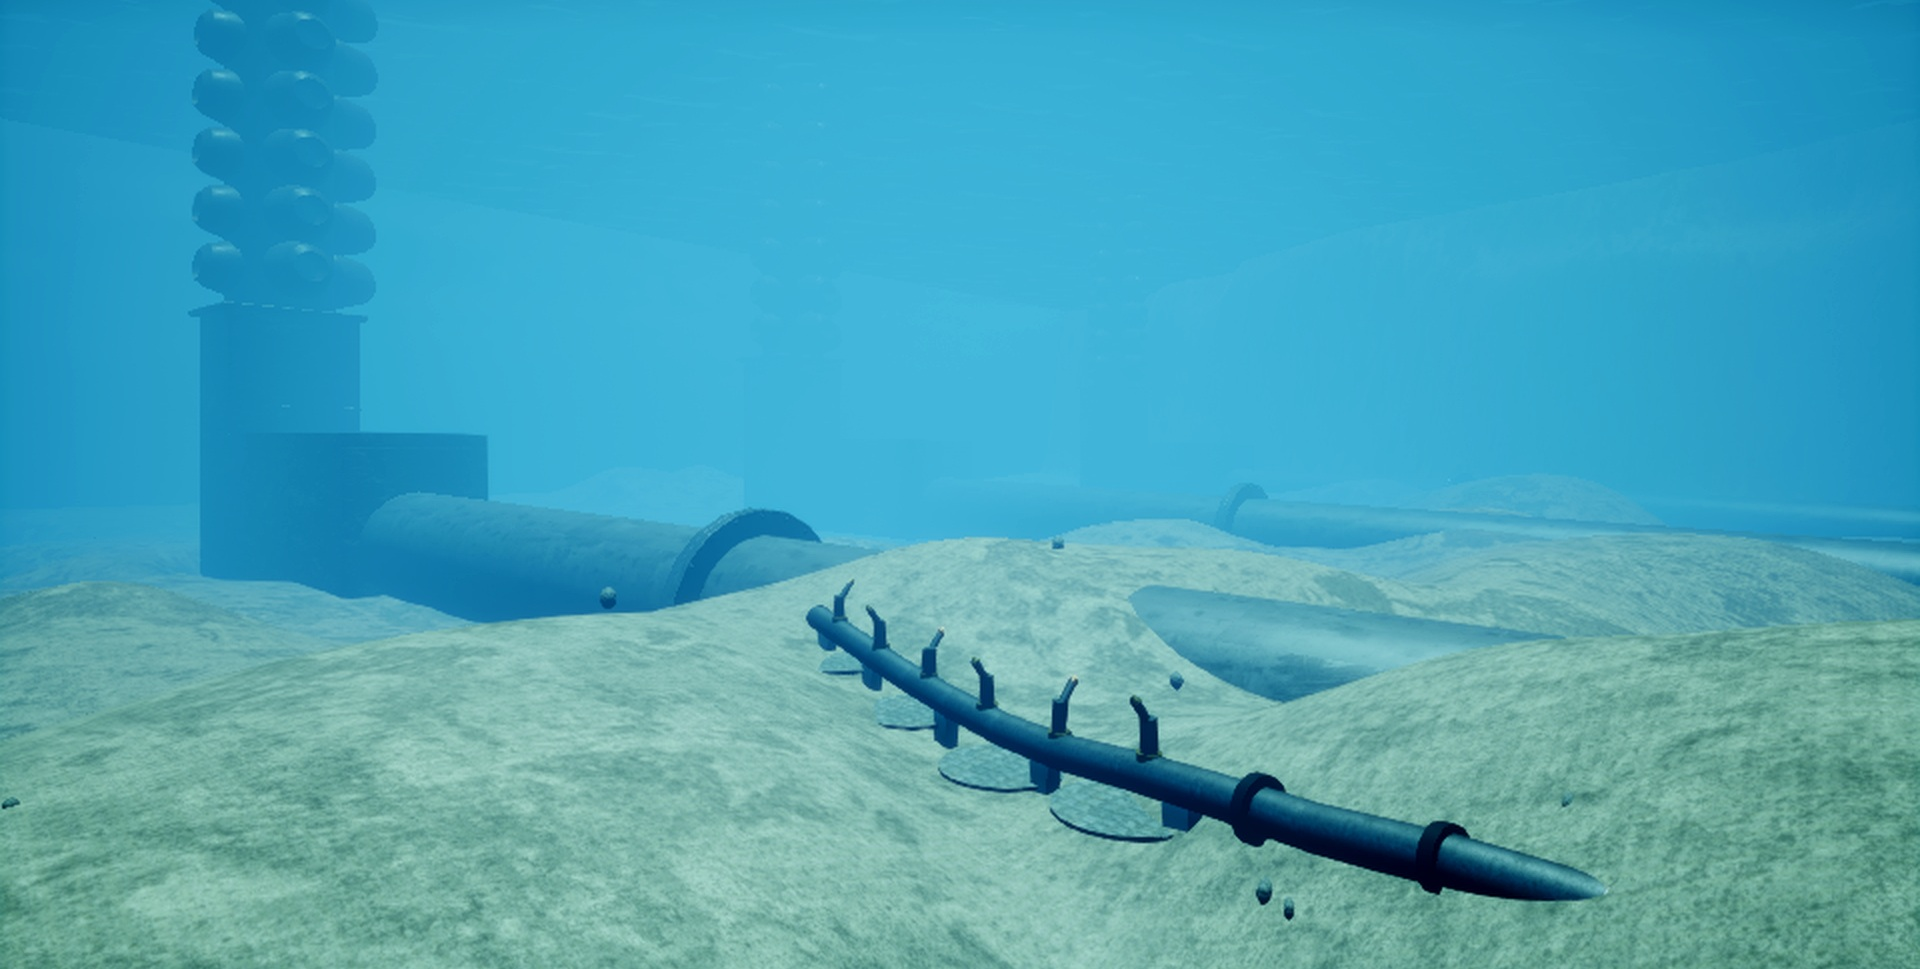
\includegraphics[width=\paperwidth,height=10.6cm,keepaspectratio=false]{figures/hero_wide.jpg}};
  \fill[deepblue] ([yshift=-10.6cm]current page.north west) rectangle
                  ([yshift=-10.72cm]current page.north east);
  \fill[teal] ([yshift=-10.6cm,xshift=0cm]current page.north west) rectangle
              ([yshift=-10.72cm,xshift=6.4cm]current page.north west);
\end{tikzpicture}

\vspace*{9.55cm}

{\sffamily\bfseries\fontsize{44}{46}\selectfont\color{deepblue}BrineWatch}\\[6pt]
{\sffamily\fontsize{15.5}{19}\selectfont\color{navy}Seeing what desalination leaves on the seabed}\\[2pt]
{\sffamily\fontsize{10.5}{14}\selectfont\color{muted}An underwater robotic system for outfall inspection and brine-plume mapping}

\vspace{13pt}
{\fontsize{12.5}{17}\selectfont\itshape\color{deepblue}%
An underwater robot that locates desalination outfalls, maps the invisible brine plume around them
and tells operators where environmental sampling matters most, turning a routine inspection dive
into actionable environmental evidence.}

\vspace{15pt}
\begin{panel}
\sffamily\small
\begin{tabularx}{\linewidth}{@{}>{\color{muted}}p{3.45cm}>{\color{navy}}X@{}}
Applicant \& team lead & \textbf{Andrea Bedei}, PhD student, University of Bologna \\[1.5pt]
Academic supervisors & Roberto Girau \textperiodcentered\ Giovanni Pau \textperiodcentered\ University of Bologna \\[1.5pt]
Project collaborators & Lorenzo Bacchiani \textperiodcentered\ Andrea Melis \\[1.5pt]
Project phase & \textbf{Simulation Prototype or Model} \\[1.5pt]
Submission & Prototypes for Humanity 2026 \\
\end{tabularx}
\end{panel}

\vfill
{\sffamily\footnotesize\color{muted}Cover image: the simulated outfall diffuser and inspection scene used to develop and
test the full BrineWatch mission.}

\clearpage
% ============================================================
% PAGE 2 — THE PROBLEM
% ============================================================
\setcounter{section}{0}
\section{The problem: fresh water's invisible waste stream}

More than 300 million people drink water that comes from the sea. Desalination keeps entire
regions alive. It is growing fast in the Gulf and increasingly across the Mediterranean.
But every litre of fresh water leaves behind roughly 1.5~litres of \keyword{brine}: seawater
concentrated to nearly twice its natural salinity, often warmer, discharged back into the sea
through submarine outfalls, amounting to about \keyword{142 million m\textsuperscript{3} every day}
worldwide, more than half of it in the Gulf region alone~[1].

The physics is what makes this problem invisible. Brine is \emph{denser} than seawater: after
leaving the diffuser it sinks, collapses onto the seabed and creeps along the bottom as a slow
salty layer~[2]. That is exactly where seagrass meadows, shellfish and the base of coastal food
chains live. This is exactly where nobody is looking. \keyword{Satellites see only the surface.
Fixed buoys measure one point, usually at the wrong depth. Survey vessels visit a few times a
year.} Between visits, the plume moves with tides and currents, unobserved.

\begin{figure}[h!]
\centering
\resizebox{\textwidth}{!}{%
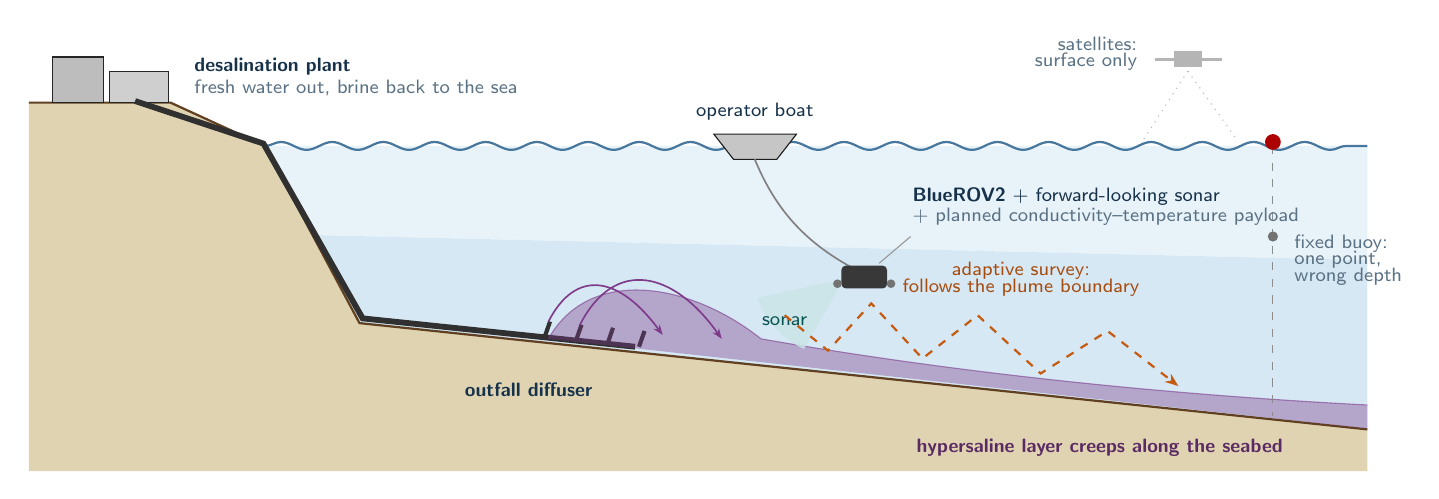
\begin{tikzpicture}[x=1cm,y=1cm,font=\scriptsize\sffamily]
  % ---- water body ----
  \fill[waterc!55] (3.0,4.55) -- (17.0,4.55) -- (17.0,3.1) -- (3.55,3.42) -- cycle;
  \fill[waterc] (3.55,3.42) -- (17.0,3.1) -- (17.0,0.95) -- (4.2,2.3) -- cycle;
  \fill[waterc!80] (3.0,4.55) -- (4.2,2.3) -- (3.0,2.42) -- cycle;
  % ---- land + seabed ----
  \fill[landc] (0,5.1) -- (1.8,5.1) -- (3.0,4.55) -- (4.2,2.3) -- (17.0,0.95) -- (17.0,0.42) -- (0,0.42) -- cycle;
  \draw[brown!50!black,thick] (0,5.1) -- (1.8,5.1) -- (3.0,4.55) -- (4.2,2.3) -- (17.0,0.95);
  % ---- sea surface ----
  \draw[deepblue!75,thick,decorate,decoration={snake,amplitude=0.05cm,segment length=0.65cm}]
      (3.0,4.55) -- (17.0,4.55);
  % ---- desalination plant ----
  \fill[gray!52] (0.30,5.1) rectangle (0.95,5.68);
  \fill[gray!38] (1.02,5.1) rectangle (1.78,5.50);
  \draw[gray!30!black] (0.30,5.1) rectangle (0.95,5.68);
  \draw[gray!30!black] (1.02,5.1) rectangle (1.78,5.50);
  \node[anchor=west,align=left,color=navy] at (1.98,5.56) {\textbf{desalination plant}};
  \node[anchor=west,align=left,color=muted] at (1.98,5.28) {fresh water out, brine back to the sea};
  % ---- outfall pipe + diffuser ----
  \draw[line width=2.1pt,gray!38!black] (1.35,5.12) -- (2.98,4.58) -- (4.24,2.36) -- (7.7,2.0);
  \foreach \x/\y in {6.55/2.12, 6.95/2.08, 7.35/2.04, 7.75/2.0}{
      \draw[line width=1.5pt,gray!38!black] (\x,\y) -- ($(\x,\y)+(0.07,0.2)$);}
  \node[anchor=north,align=center,color=navy] at (6.35,1.66) {\textbf{outfall diffuser}};
  % ---- brine jets ----
  \draw[-{Stealth[length=1.3mm]},brine,semithick] (6.6,2.32) .. controls (6.95,3.0) and (7.5,2.9) .. (8.05,2.15);
  \draw[-{Stealth[length=1.3mm]},brine,semithick] (7.0,2.28) .. controls (7.45,3.15) and (8.2,2.95) .. (8.8,2.1);
  % ---- plume gravity current ----
  \fill[brine,fill opacity=0.38] (6.6,2.1)
      .. controls (7.1,3.0) and (8.35,2.85) .. (9.3,2.1)
      .. controls (11.3,1.75) and (13.9,1.42) .. (17.0,1.26)
      -- (17.0,0.96) -- cycle;
  \draw[brine,opacity=0.6,thin] (6.6,2.1)
      .. controls (7.1,3.0) and (8.35,2.85) .. (9.3,2.1)
      .. controls (11.3,1.75) and (13.9,1.42) .. (17.0,1.26);
  \node[align=left,anchor=west,text=brine!72!black] at (11.15,0.72)
      {\textbf{hypersaline layer creeps along the seabed}};
  % ---- satellite ----
  \fill[gray!58] (14.55,5.55) rectangle (14.9,5.75);
  \draw[gray!58,line width=1pt] (14.3,5.65) -- (14.55,5.65) (14.9,5.65) -- (15.15,5.65);
  \draw[dotted,gray!55] (14.72,5.5) -- (14.15,4.62) (14.72,5.5) -- (15.35,4.62);
  \node[anchor=east,align=right,color=muted] at (14.2,5.72) {satellites:\\[-2pt]surface only};
  % ---- fixed buoy ----
  \draw[dashed,black!45] (15.8,4.55) -- (15.8,1.12);
  \fill[red!68!black] (15.8,4.6) circle (0.1);
  \fill[black!55] (15.8,3.4) circle (0.065);
  \node[anchor=west,align=left,color=muted] at (15.95,3.1) {fixed buoy:\\[-2pt]one point,\\[-2pt]wrong depth};
  % ---- operator boat + tether ----
  \fill[gray!45] (8.7,4.7) -- (9.75,4.7) -- (9.5,4.38) -- (8.95,4.38) -- cycle;
  \draw[gray!22!black] (8.7,4.7) -- (9.75,4.7) -- (9.5,4.38) -- (8.95,4.38) -- cycle;
  \node[anchor=south,color=navy] at (9.22,4.75) {operator boat};
  \draw[black!50,semithick] (9.22,4.38) .. controls (9.5,3.7) and (9.9,3.3) .. (10.5,2.98);
  % ---- ROV + sonar wedge ----
  \fill[teal!22,opacity=.85] (10.35,2.86) -- (9.25,2.62) arc (200:245:1.15) -- cycle;
  \fill[rounded corners=1.6pt,black!78] (10.32,2.74) rectangle (10.9,3.03);
  \fill[black!55] (10.27,2.8) circle (0.055);
  \fill[black!55] (10.95,2.8) circle (0.055);
  \node[anchor=south west,align=left,color=navy] at (11.1,3.42)
      {\textbf{BlueROV2} + forward-looking sonar\\[-1pt]{\color{muted}+ planned conductivity--temperature payload}};
  \draw[black!40,thin] (11.2,3.4) -- (10.8,3.06);
  \node[anchor=north,align=center,color=teal!60!black] at (9.6,2.5) {sonar};
  % ---- adaptive trajectory ----
  \draw[dashed,accent,thick,-{Stealth[length=1.7mm]}]
      (9.6,2.4) -- (10.15,1.95) -- (10.7,2.55) -- (11.35,1.85) -- (12.05,2.4)
      -- (12.85,1.66) -- (13.7,2.2) -- (14.6,1.5);
  \node[anchor=south,align=center,color=accent!85!black] at (12.6,2.52) {adaptive survey:\\[-2pt]follows the plume boundary};
\end{tikzpicture}}

\vspace{5pt}
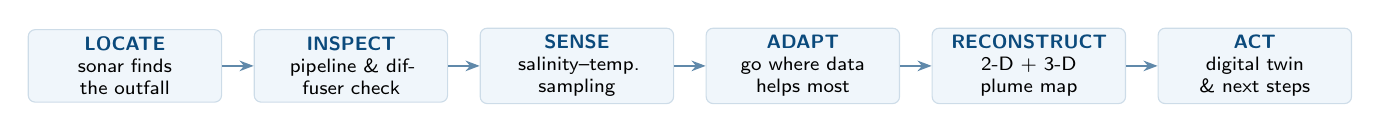
\begin{tikzpicture}[font=\scriptsize\sffamily,
    box/.style={draw=hairline,fill=panelblue,rounded corners=2.5pt,align=center,
                minimum height=0.92cm,text width=2.28cm,inner sep=2.5pt},
    arr/.style={-{Stealth[length=1.8mm]},deepblue!65,semithick}]
  \node[box] (a) at (0,0)     {\textbf{\color{deepblue}LOCATE}\\sonar finds the outfall};
  \node[box] (b) at (2.87,0)  {\textbf{\color{deepblue}INSPECT}\\pipeline \& diffuser check};
  \node[box] (c) at (5.74,0)  {\textbf{\color{deepblue}SENSE}\\salinity--temp.\ sampling};
  \node[box] (d) at (8.61,0)  {\textbf{\color{deepblue}ADAPT}\\go where data helps most};
  \node[box] (e) at (11.48,0) {\textbf{\color{deepblue}RECONSTRUCT}\\2-D + 3-D plume map};
  \node[box] (f) at (14.35,0) {\textbf{\color{deepblue}ACT}\\digital twin \& next steps};
  \draw[arr] (a) -- (b); \draw[arr] (b) -- (c); \draw[arr] (c) -- (d);
  \draw[arr] (d) -- (e); \draw[arr] (e) -- (f);
\end{tikzpicture}
\caption{\textbf{The BrineWatch mission at a glance.} Dense brine sinks and spreads along the seabed,
where satellites, buoys and quarterly boat surveys cannot follow it. BrineWatch sends a small robot
along the plume itself: it finds the outfall with sonar, inspects the structure, samples salinity
where it is most informative and returns a mapped, uncertainty-aware picture of the discharge zone.}
\label{fig:concept}
\end{figure}

\begin{panel}
\sffamily\small\textbf{\color{deepblue}Who feels this problem}\quad
\textcolor{navy}{Desalination plant operators \textperiodcentered\ environmental regulators
\textperiodcentered\ marine survey companies \textperiodcentered\ coastal authorities
\textperiodcentered\ research laboratories}
\end{panel}

\clearpage
% ============================================================
% PAGE 3 — WHY CURRENT MONITORING IS LIMITED
% ============================================================
\section{Why today's monitoring falls short}

Discharge permits define a \keyword{mixing zone}: a distance from the diffuser beyond which
salinity must return close to ambient. Verifying it requires spatial information: where the plume
actually goes. Yet routine monitoring still relies on tools that were never designed to answer a
spatial question:

\begin{itemize}
  \item \keyword{Fixed stations}: accurate, but only at a handful of points that the plume can simply miss;
  \item \keyword{Manual probe casts}: a technician lowers an instrument from a boat, station by station;
  \item \keyword{Vessel campaigns}: thorough but expensive, so they happen every few months;
  \item \keyword{Static reports}: results arrive weeks later, describing a sea state that has already changed.
\end{itemize}

The result: operators and regulators work with a few dozen correct numbers that may still
miss the plume between them.

\vspace{4pt}
\noindent
\begin{minipage}[t]{0.485\textwidth}
\begin{panel}
{\sffamily\bfseries\color{muted}TODAY'S WORKFLOW}\\[4pt]
\small
\begin{itemize}
  \item sparse point measurements
  \item fixed locations, chosen in advance
  \item vessel campaign every 3--6 months
  \item results reported weeks later
  \item little or no usable site history
\end{itemize}
\end{panel}
\end{minipage}\hfill
\begin{minipage}[t]{0.485\textwidth}
\begin{tealpanel}
{\sffamily\bfseries\color{teal}THE BRINEWATCH WORKFLOW}\\[4pt]
\small
\begin{itemize}
  \item mobile measurements along the plume
  \item survey adapts to what it finds
  \item inspection + environment in one mission
  \item map with explicit uncertainty, same day
  \item repeatable digital site history
\end{itemize}
\end{tealpanel}
\end{minipage}

\subsection*{\sffamily\color{deepblue}What changes in practice}

Consider the routine question: \emph{``is the discharge behaving as permitted?''} Today the
answer depends on whether a handful of fixed points happened to intersect the plume. With
BrineWatch, one robot mission produces a picture: where the outfall is, the condition of the
diffuser, a salinity map around it with a clear boundary estimate, the parts of the site that
remain uncertain and a concrete recommendation of where to send the certified sampling team
next. The mission is repeatable, so each visit adds a page to the same site history rather than
starting from zero.

\begin{figure}[h!]
\centering
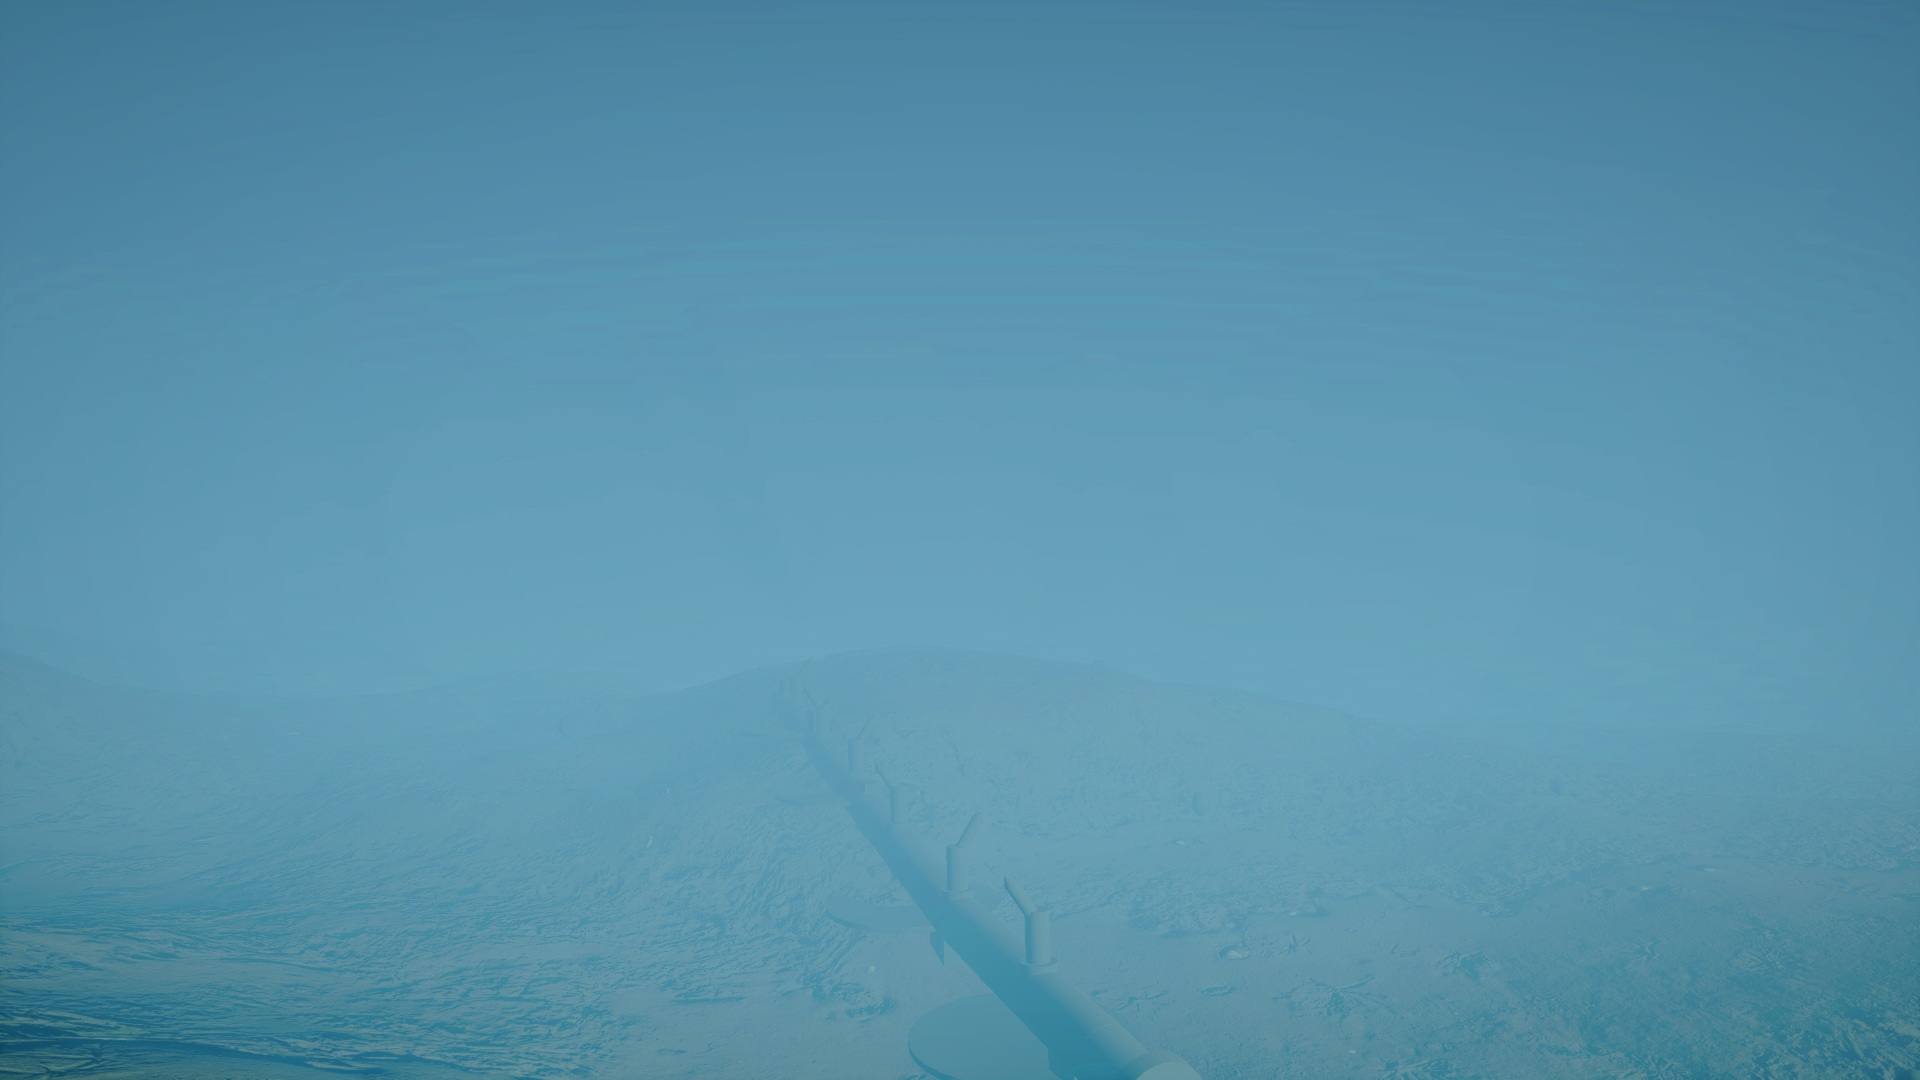
\includegraphics[width=\textwidth]{figures/still_approach.jpg}
\caption{\textbf{Approaching the outfall.} A frame from the project's simulated inspection
mission: the pipeline and diffuser risers emerge from the haze as the vehicle approaches.
This is the moment monitoring stops being blind.}
\end{figure}

\clearpage
% ============================================================
% PAGE 4 — THE BRINEWATCH SYSTEM
% ============================================================
\section{The BrineWatch system}

BrineWatch is built deliberately from accessible parts: a proven open-source inspection robot,
one commercial imaging sonar, one scientific sensor and software that turns them into an
autonomous environmental instrument.

\begin{figure}[h!]
\centering
\begin{tikzpicture}[font=\scriptsize\sffamily,
  hw/.style={draw=hairline,fill=panelblue,rounded corners=3pt,align=center,inner sep=5pt},
  hwplan/.style={draw=accent!70,dashed,fill=panelwarm,rounded corners=3pt,align=center,inner sep=5pt},
  sw/.style={draw=hairline,fill=panelteal,rounded corners=3pt,align=center,inner sep=5pt},
  lab/.style={color=muted,align=center},
  arr/.style={-{Stealth[length=1.8mm]},deepblue!60,semithick}]

  % vehicle group
  \node[hw,minimum width=4.35cm,minimum height=1.02cm] (rov) at (0,0)
    {\textbf{\color{deepblue}\faRobot~~BlueROV2}\\vehicle \textperiodcentered\ camera \textperiodcentered\ lights \textperiodcentered\ depth \& heading};
  \node[hw,minimum width=4.35cm] (sonar) at (0,-1.28)
    {\textbf{\color{deepblue}\faWifi~~Omniscan 450 FS}\\forward-looking imaging sonar};
  \node[hwplan,minimum width=4.35cm] (ct) at (0,-2.48)
    {\textbf{\color{accent}\faTint~~CT payload (planned)}\\calibrated conductivity--temperature};
  \node[lab] at (0,-3.35) {\footnotesize ON THE VEHICLE};

  % topside group
  \node[sw,minimum width=4.5cm] (planner) at (6.6,0)
    {\textbf{\color{teal}\faRoute~~Mission planner}\\adaptive waypoints, collision-safe};
  \node[sw,minimum width=4.5cm] (gp) at (6.6,-1.28)
    {\textbf{\color{teal}\faChartArea~~Field reconstruction}\\2-D + 3-D salinity map with uncertainty};
  \node[sw,minimum width=4.5cm] (twin) at (6.6,-2.48)
    {\textbf{\color{teal}\faHistory~~Digital twin}\\site record, screening state, next action};
  \node[lab] at (6.6,-3.35) {\footnotesize MISSION SOFTWARE (RUNS TOPSIDE)};

  % operator
  \node[hw,minimum width=3.3cm,minimum height=1.02cm] (op) at (12.35,0)
    {\textbf{\color{deepblue}\faDesktop~~Operator}\\dashboard \& mission control};
  \node[hw,minimum width=3.3cm] (out) at (12.35,-2.48)
    {\textbf{\color{deepblue}\faClipboardCheck~~Site report}\\map \textperiodcentered\ uncertainty \textperiodcentered\ recommendation};

  \draw[arr] (rov.east) -- node[above,lab,font=\tiny]{video \& telemetry} (planner.west);
  \draw[arr] (sonar.east) -- (gp.west);
  \draw[arr] (ct.east) -- (twin.west);
  \draw[arr] (planner.east) -- (op.west);
  \draw[arr] (twin.east) -- (out.west);
  \draw[arr,{Stealth[length=1.8mm]}-{Stealth[length=1.8mm]}] (planner.south) -- (gp.north);
  \draw[arr,{Stealth[length=1.8mm]}-{Stealth[length=1.8mm]}] (gp.south) -- (twin.north);
\end{tikzpicture}
\caption{\textbf{System overview.} Solid blue panels: hardware available today. Dashed panel:
the calibrated CT sensor, the next integration step. Teal panels: mission software already
implemented and exercised in simulation.}
\end{figure}

\vspace{-2pt}
\noindent
\begin{minipage}[t]{0.485\textwidth}
\begin{tealpanel}[height=3.6cm,valign=top]
{\sffamily\bfseries\color{teal}ALREADY IN PLACE}\\[3pt]
\small
\begin{itemize}
  \item BlueROV2 owned by the team
  \item full mission software: planning, sonar localisation, mapping, digital twin
  \item high-fidelity simulation environment (custom HoloOcean fork, Unreal Engine)
  \item complete simulated missions with video evidence
\end{itemize}
\end{tealpanel}
\end{minipage}\hfill
\begin{minipage}[t]{0.485\textwidth}
\begin{warmpanel}[height=3.6cm,valign=top]
{\sffamily\bfseries\color{accent}NEXT INTEGRATION STEPS}\\[3pt]
\small
\begin{itemize}
  \item validation in controlled water, then at sea
\end{itemize}
\end{warmpanel}
\end{minipage}

\begin{figure}[h!]
\centering
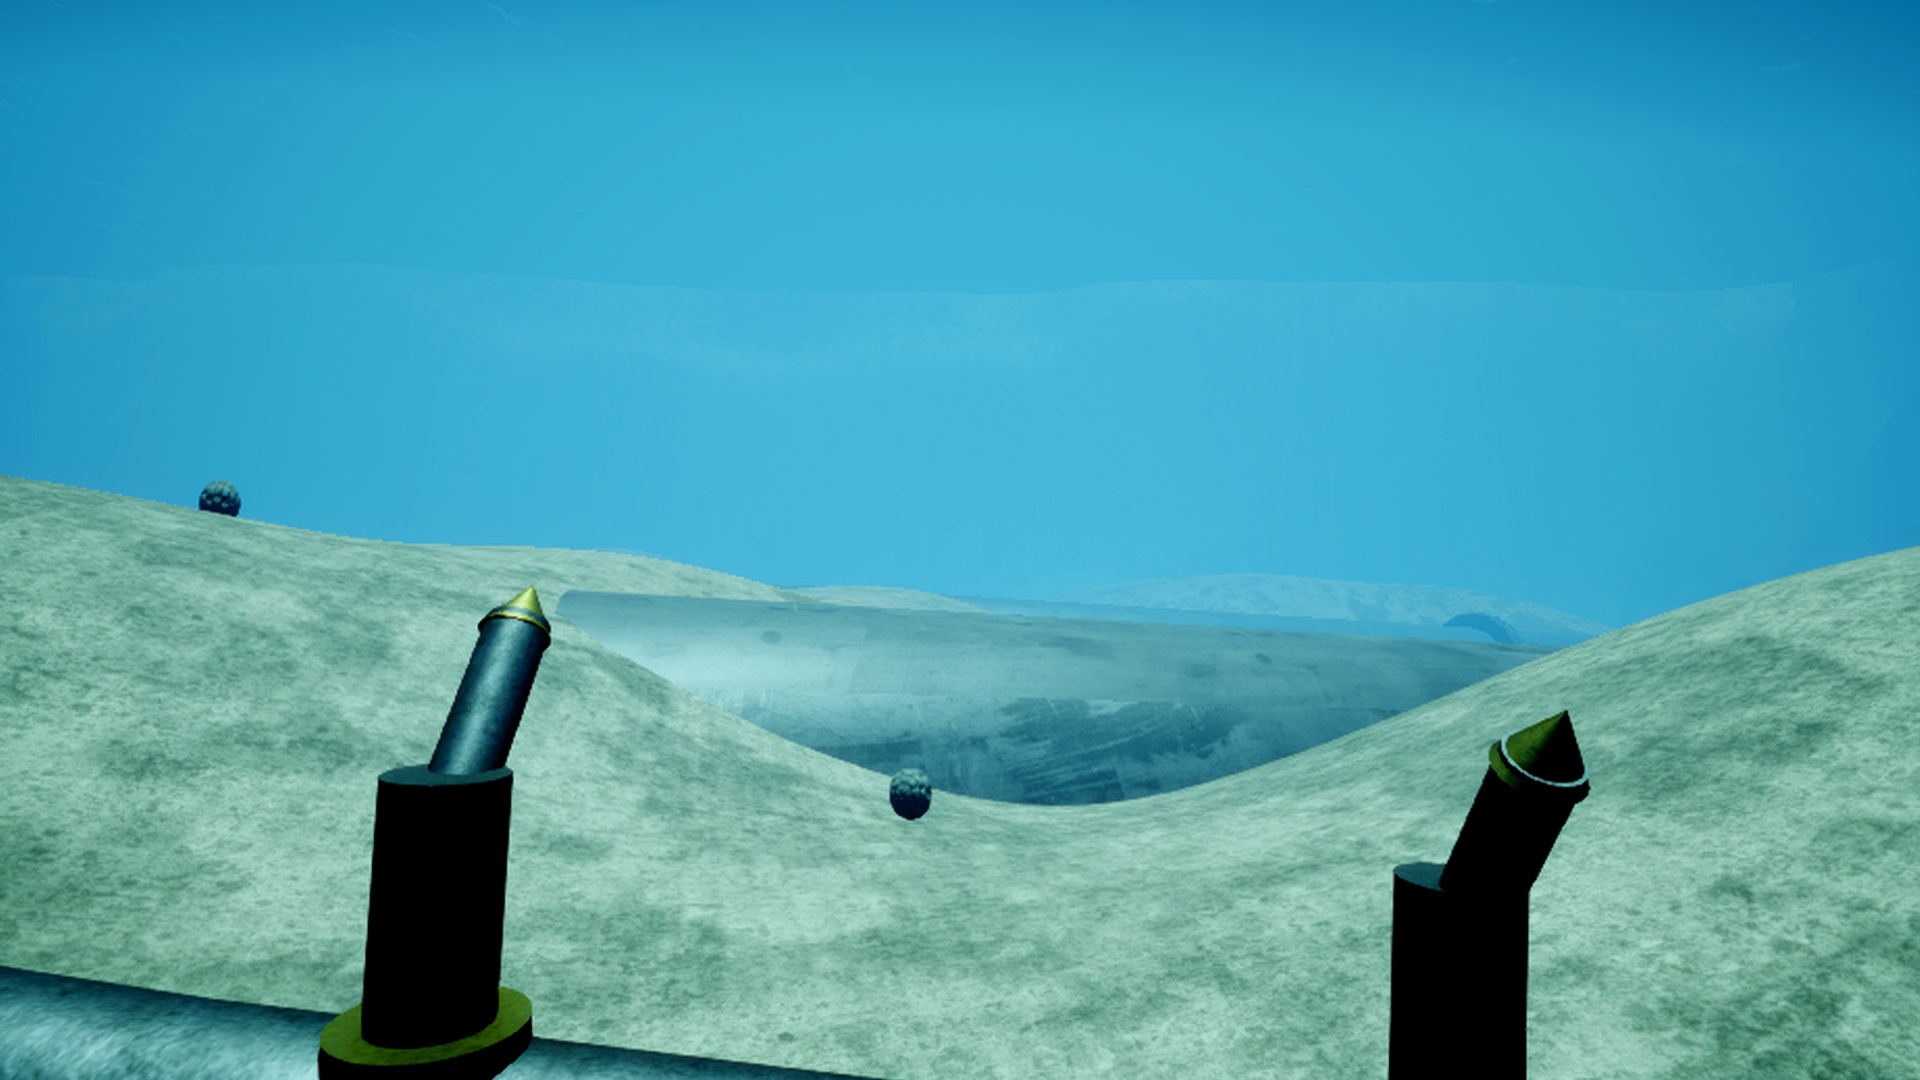
\includegraphics[width=\textwidth]{figures/hero_closeup.jpg}
\caption{\textbf{Inside the simulation.} The diffuser risers seen from the vehicle during a
simulated inspection pass.}
\end{figure}

\clearpage
% ============================================================
% PAGE 5 — HOW A MISSION WORKS
% ============================================================
\section{How a mission works}

Every BrineWatch mission follows the same six movements: simple enough to brief a crew in a
morning, rich enough to produce evidence a regulator can use.

\newcommand{\stepbox}[3]{%
\begin{minipage}[t]{0.318\textwidth}
\begin{panel}[left=7pt,right=7pt,top=6pt,bottom=6pt,height=2.9cm,valign=top]
{\sffamily\bfseries\color{deepblue}#1~~#2}\\[2.5pt]
{\small #3}
\end{panel}
\end{minipage}}

\noindent
\stepbox{\faSearchLocation}{LOCATE}{The forward-looking sonar finds the outfall on the seabed and anchors the whole survey to it. No GPS exists underwater.}\hfill
\stepbox{\faVideo}{INSPECT}{The vehicle follows the pipeline to the diffuser, checking risers and nozzles with camera and sonar, at a safe standoff.}\hfill
\stepbox{\faTint}{SENSE}{The CT payload records salinity, temperature and depth continuously along the route.}

\vspace{2pt}
\noindent
\stepbox{\faRoute}{ADAPT}{After each leg, the planner asks: \emph{where would the next reading teach us most?} It then routes the vehicle there.}\hfill
\stepbox{\faCubes}{RECONSTRUCT}{All samples fuse into 2-D and 3-D salinity maps with an explicit confidence level for every location.}\hfill
\stepbox{\faClipboardCheck}{ACT}{The digital twin stores the mission, raises a clear screening state and recommends where certified sampling should go next.}

\begin{figure}[h!]
\centering
\begin{minipage}[t]{0.492\textwidth}
  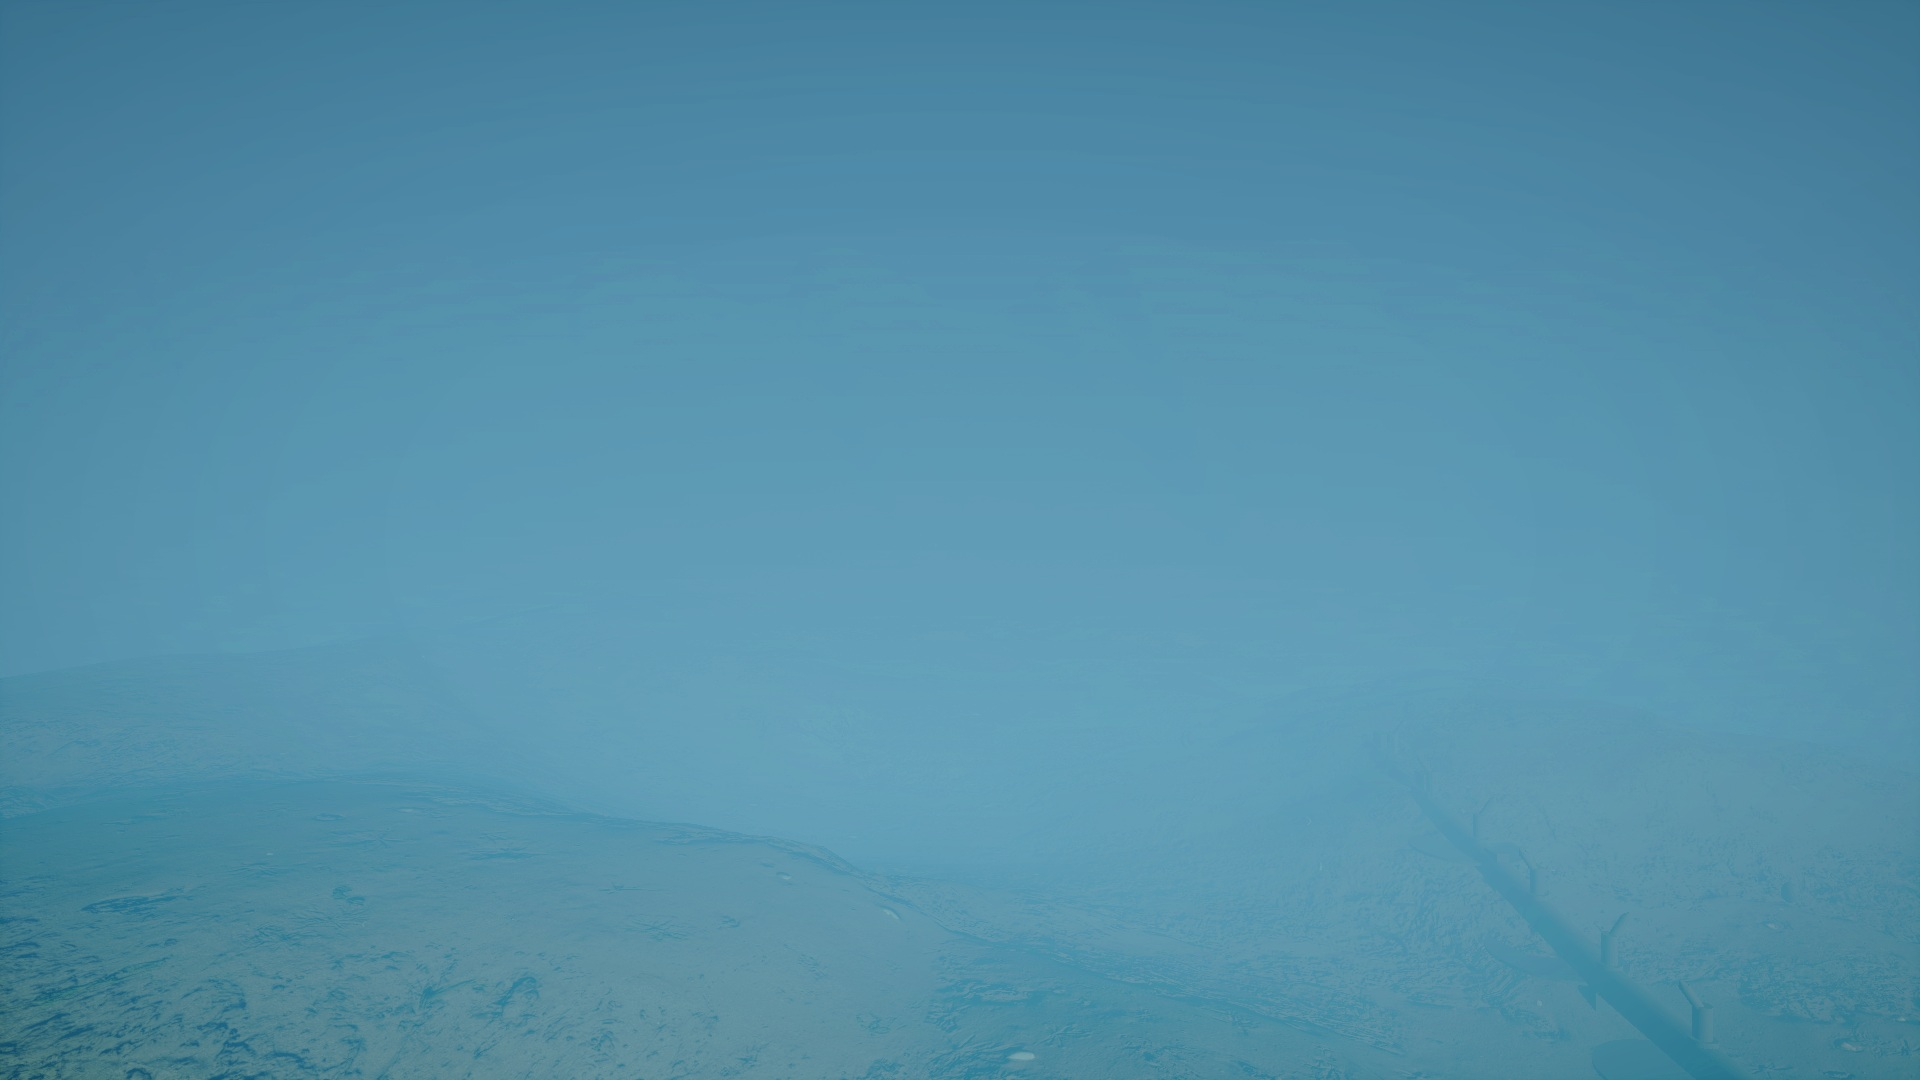
\includegraphics[width=\linewidth]{figures/still_descent.jpg}
\end{minipage}\hfill
\begin{minipage}[t]{0.492\textwidth}
  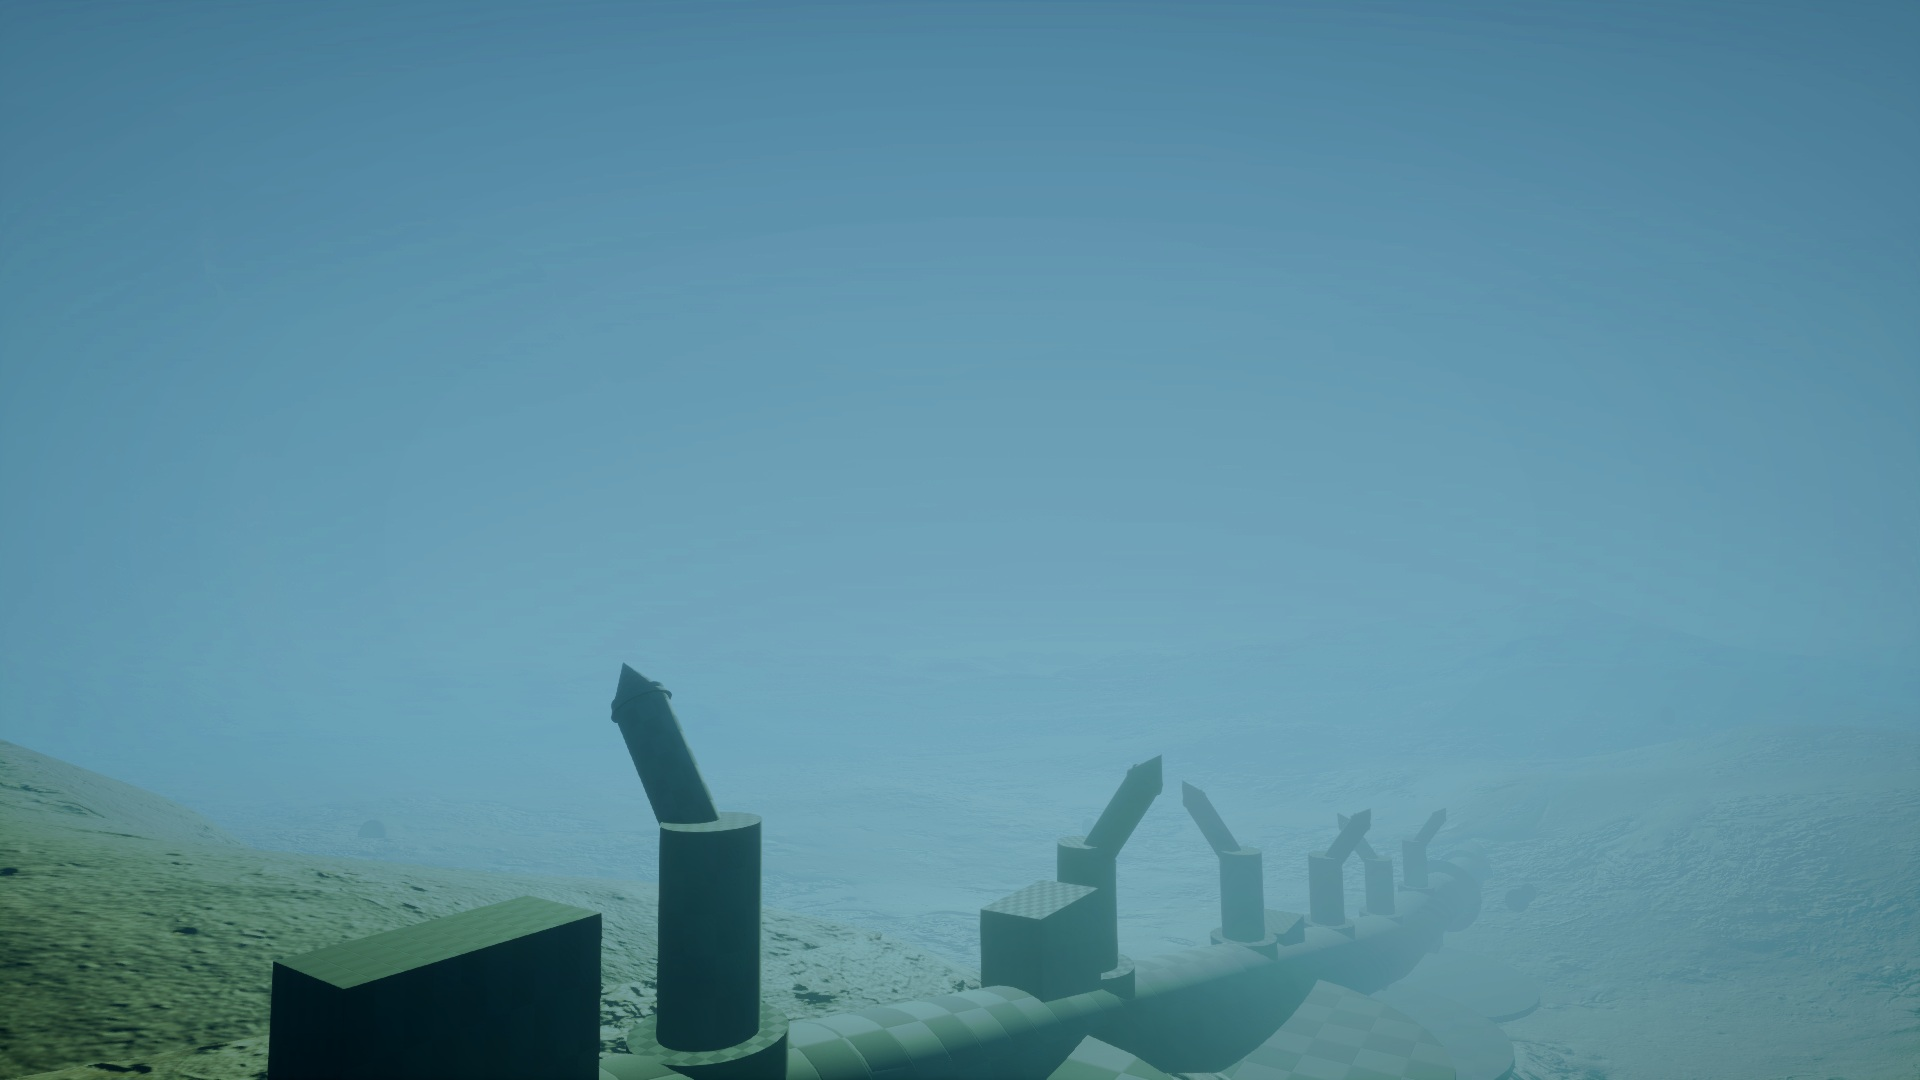
\includegraphics[width=\linewidth]{figures/still_nozzles.jpg}
\end{minipage}\\[5pt]
\begin{minipage}[t]{0.492\textwidth}
  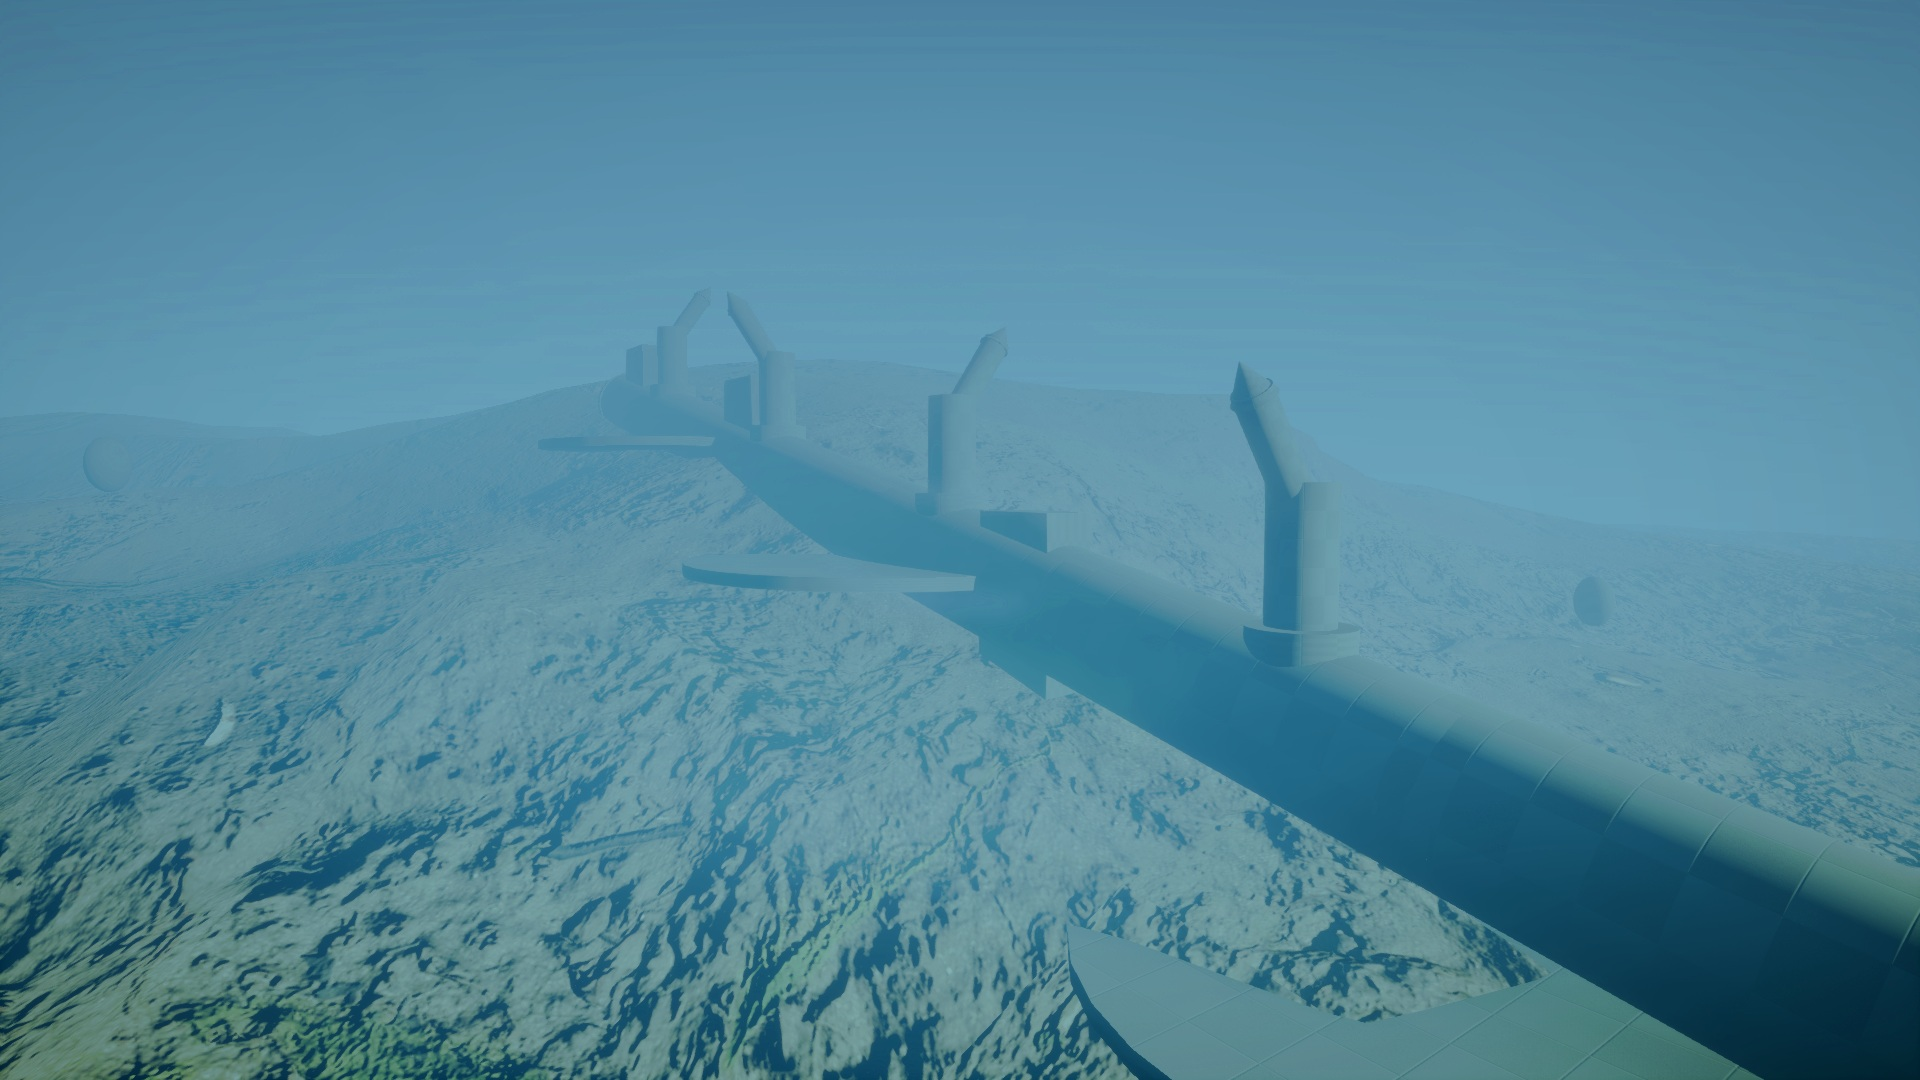
\includegraphics[width=\linewidth]{figures/still_inspect.jpg}
\end{minipage}\hfill
\begin{minipage}[t]{0.492\textwidth}
  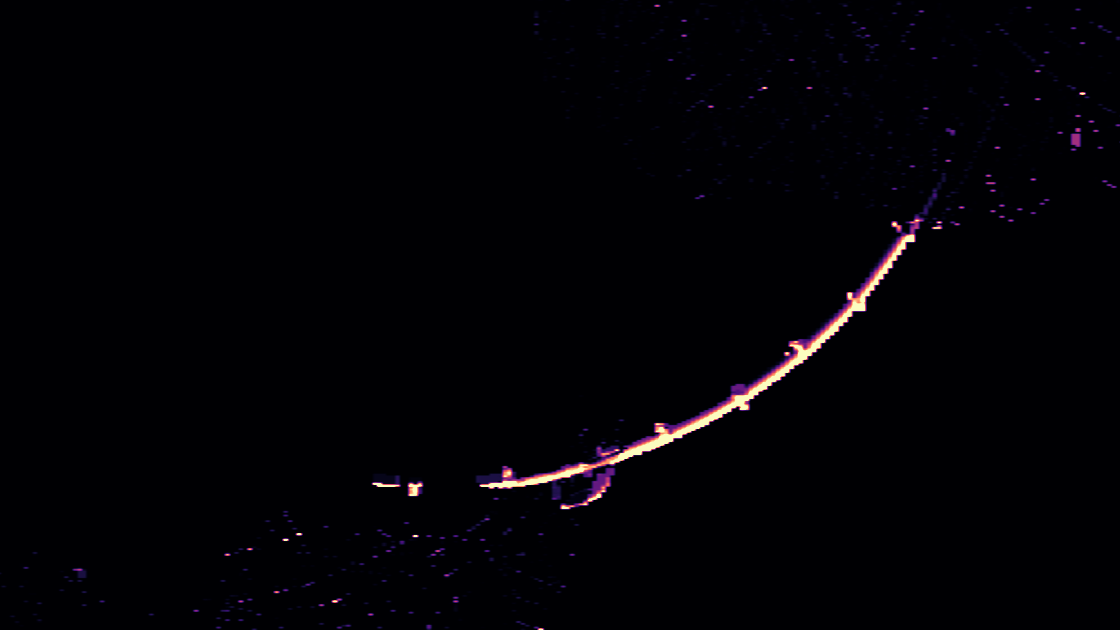
\includegraphics[width=\linewidth]{figures/sonar_residual.png}
\end{minipage}
\caption{\textbf{One continuous simulated mission.} Clockwise from top left: descent to the site;
close pass over the diffuser nozzles; the sonar's view, where the bright arc is the outfall structure
as the localisation algorithm sees it; following the pipeline during inspection. All frames come
from the same in-engine mission that produced the evidence in Section~6.}
\end{figure}

\clearpage
% ============================================================
% PAGE 6 — THE DIGITAL TWIN
% ============================================================
\section{What the digital twin actually is}

\emph{Digital twin} can sound like a buzzword, so here is the plain meaning:
\begin{center}
{\fontsize{12}{15}\selectfont\itshape\color{deepblue}%
The BrineWatch digital twin is the evolving operational record of one outfall site.}
\end{center}
It is not a decorative 3-D graphic. It is a structured, queryable memory: every mission adds its
sonar fix, its samples, its route, its reconstructed maps and its conclusions to the same record.
The site's story accumulates instead of evaporating into filed-away PDFs.

\begin{figure}[h!]
\centering
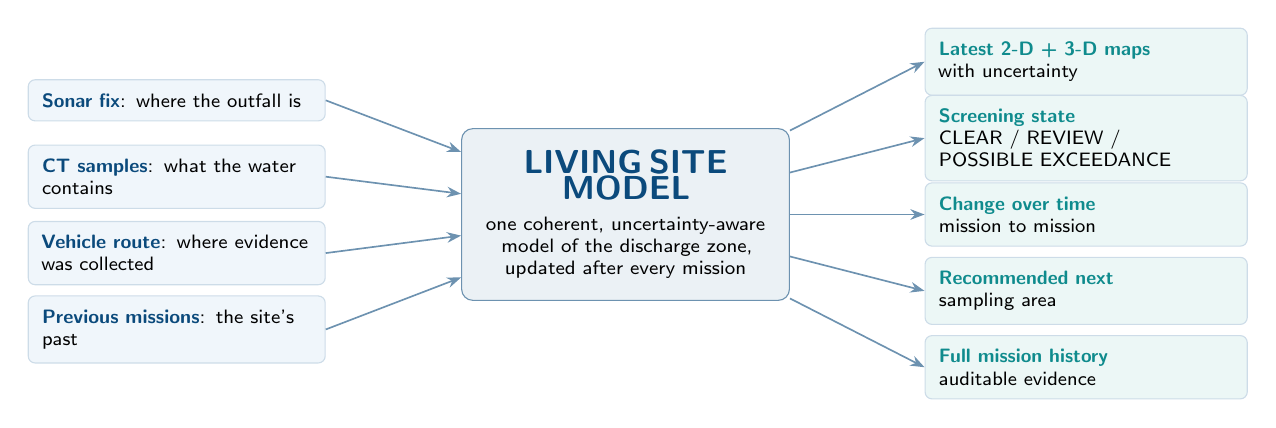
\begin{tikzpicture}[font=\scriptsize\sffamily,
  inbox/.style={draw=hairline,fill=panelblue,rounded corners=2.5pt,align=left,
                text width=3.42cm,inner sep=5pt},
  outbox/.style={draw=hairline,fill=panelteal,rounded corners=2.5pt,align=left,
                text width=3.74cm,inner sep=5pt},
  core/.style={draw=deepblue!60,fill=deepblue!8,rounded corners=4pt,align=center,
                text width=3.6cm,inner sep=8pt},
  arr/.style={-{Stealth[length=1.8mm]},deepblue!60,semithick}]
  \node[inbox] (i1) at (0,1.95)  {\textbf{\color{deepblue}Sonar fix}: where the outfall is};
  \node[inbox] (i2) at (0,0.98)  {\textbf{\color{deepblue}CT samples}: what the water contains};
  \node[inbox] (i3) at (0,0.01)  {\textbf{\color{deepblue}Vehicle route}: where evidence was collected};
  \node[inbox] (i4) at (0,-0.96) {\textbf{\color{deepblue}Previous missions}: the site's past};
  \node[core] (c) at (5.7,0.5)
    {\textbf{\color{deepblue}\large LIVING SITE MODEL}\\[3pt]
     one coherent, uncertainty-aware\\model of the discharge zone,\\updated after every mission};
  \node[outbox] (o1) at (11.55,2.44)  {\textbf{\color{teal}Latest 2-D + 3-D maps}\\with uncertainty};
  \node[outbox] (o2) at (11.55,1.47)  {\textbf{\color{teal}Screening state}\\CLEAR / REVIEW /\\POSSIBLE~EXCEEDANCE};
  \node[outbox] (o3) at (11.55,0.5)   {\textbf{\color{teal}Change over time}\\mission to mission};
  \node[outbox] (o4) at (11.55,-0.47) {\textbf{\color{teal}Recommended next}\\sampling area};
  \node[outbox] (o5) at (11.55,-1.44) {\textbf{\color{teal}Full mission history}\\auditable evidence};
  \foreach \i in {i1,i2,i3,i4} \draw[arr] (\i.east) -- (c);
  \foreach \o in {o1,o2,o3,o4,o5} \draw[arr] (c) -- (\o.west);
\end{tikzpicture}
\caption{\textbf{The twin in one picture.} Missions feed the model on the left; operators and
regulators read answers on the right.}
\end{figure}

\subsection*{\sffamily\color{deepblue}From mission data to the next action}

BrineWatch does not issue a legal pass/fail verdict. Instead, after each mission it combines the
reconstructed salinity map with its uncertainty and assigns one of three operational screening
states. \metric{CLEAR} means the plume boundary is sufficiently resolved and no elevated salinity
is indicated beyond the mixing zone, so routine monitoring can continue. \metric{REVIEW} means
the evidence remains insufficient; the uncertainty map identifies where more observations are
needed. \metric{POSSIBLE EXCEEDANCE} means elevated salinity is reconstructed beyond the
mixing-zone threshold with sufficient confidence, prompting targeted certified reference
sampling at the highest-risk location. These states support, rather than replace, regulatory
assessment by turning mission data into a clear and traceable next action.

The dashboard in Figure~\ref{fig:dashboard} presents this workflow to the operator. Its top row
summarises the current screening state and key quality indicators. The map shows the reconstructed
salinity field, estimated plume boundary and robot trajectory; the central panel highlights
uncertainty; and the right-hand panel converts the evidence into an operational recommendation.
In the example, \metric{POSSIBLE EXCEEDANCE} triggers targeted certified sampling at the
highest-risk plume-boundary location. The timeline preserves previous mission outcomes so
operators can track change over time and each survey contributes to the same digital record.

\begin{figure}[h!]
\centering
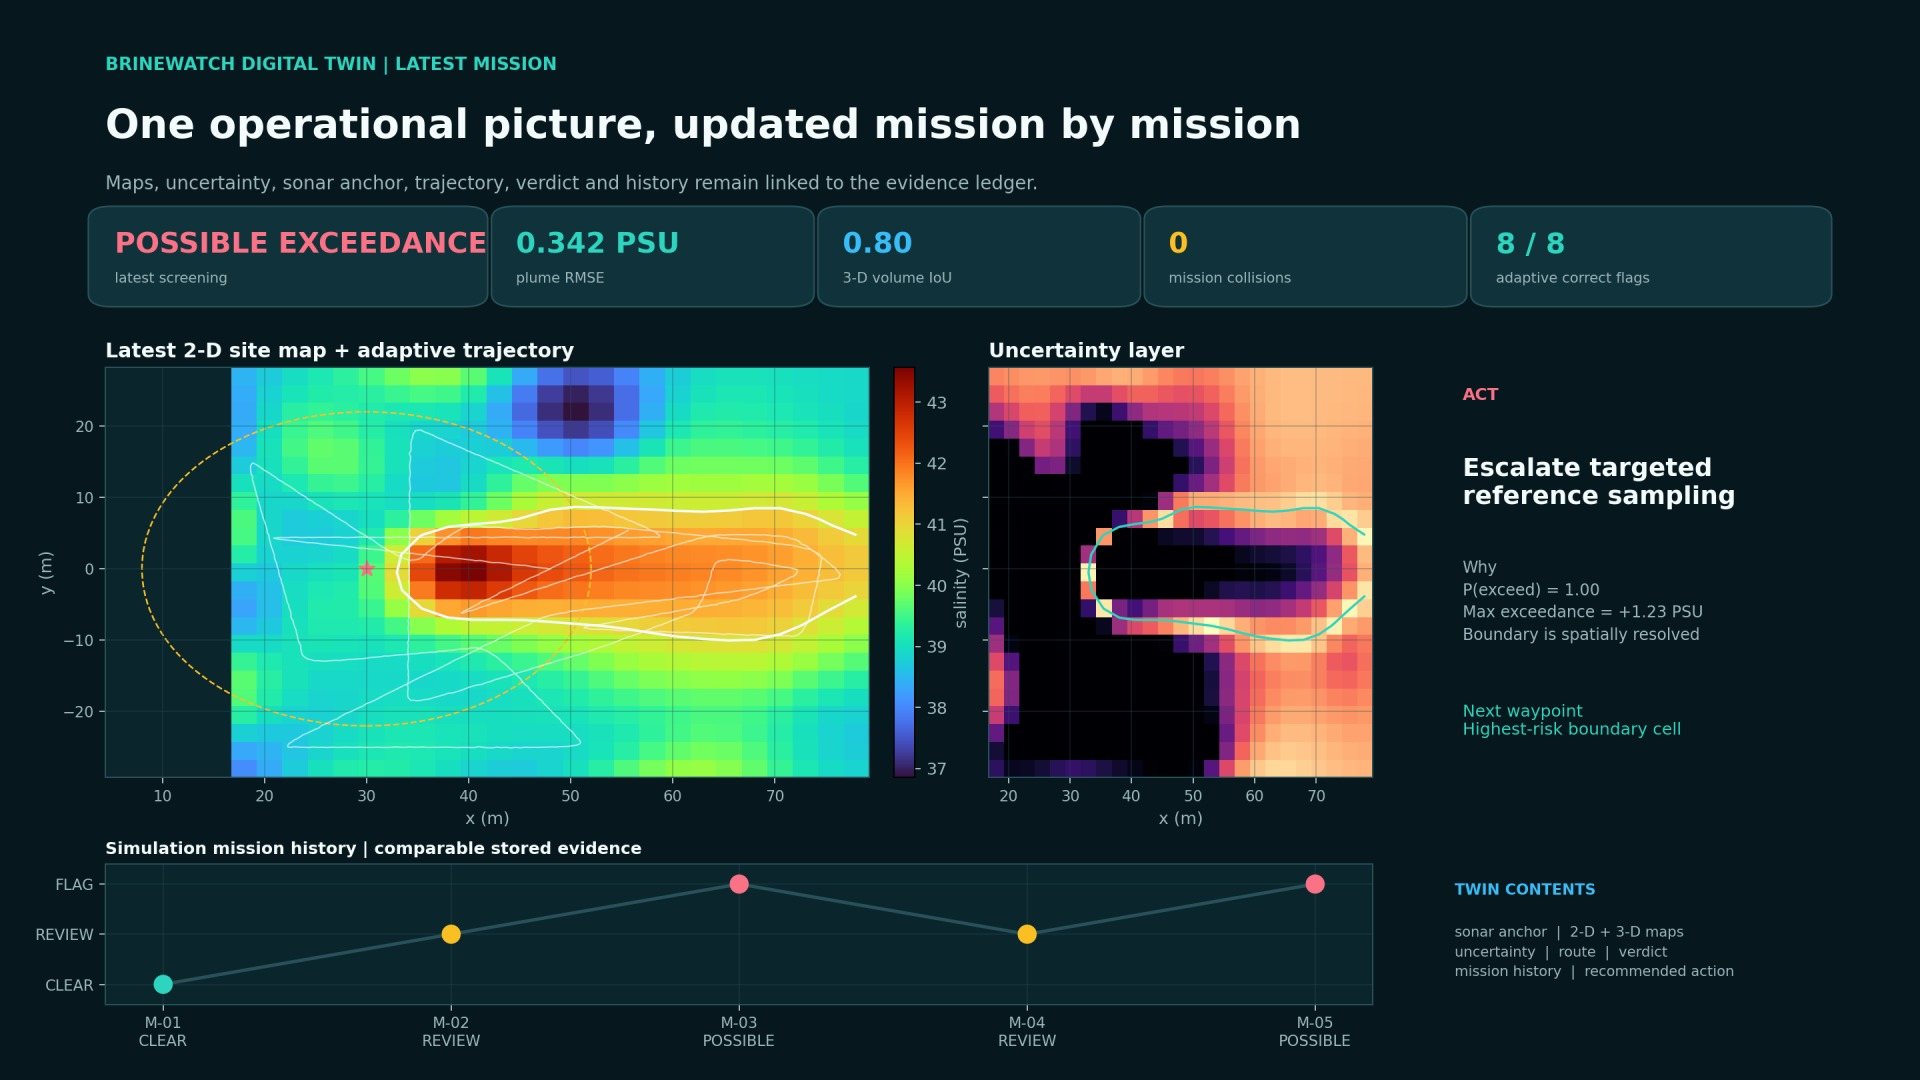
\includegraphics[width=0.84\textwidth]{figures/dashboard.jpg}
\caption{\textbf{BrineWatch operator dashboard.} The dashboard links the latest plume map,
robot trajectory, uncertainty, screening state, mission history and recommended next action in a
single operational view.}
\label{fig:dashboard}
\end{figure}

\clearpage
% ============================================================
% PAGE 7 — CURRENT PROTOTYPE AND RESULTS (A + B)
% ============================================================
\section{What has been built and what it shows}

BrineWatch today is a \keyword{simulation-led prototype}. The complete system, including vehicle
control, sonar, planning, mapping and the digital twin, runs end-to-end in a high-fidelity underwater
simulator (a custom fork of HoloOcean~[4], built on Unreal Engine).

\subsection{A full robotic mission inside the engine}

One continuous mission in the custom simulator demonstrated the complete robotic workflow using
native vehicle dynamics and native simulated sonar. Figure~\ref{fig:mission-map} isolates the
navigation sequence to make the evidence easy to read. The grey line marks the outfall structure
and the six circles mark the diffuser risers. The grey
cross is the approximate chart prior and the orange star is the sonar fix obtained by the vehicle.
From that anchor, the pale route records the baseline legs and the dark-blue route shows the
adaptive survey around the structure. This is the same mission summarised below:

\begin{center}
\sffamily\small
\begin{tabularx}{\textwidth}{@{}XXXX@{}}
\metric{\large 394.8 m} & \metric{\large 564} & \metric{\large 0} & \metric{\large 2.35 m}\\
\color{muted}travelled in-engine, within a 400 m budget & \color{muted}salinity readings collected along the route & \color{muted}collisions, with 4 safe detours around the structure & \color{muted}sonar localisation error of the diffuser\\
\end{tabularx}
\end{center}

\begin{figure}[h!]
\centering
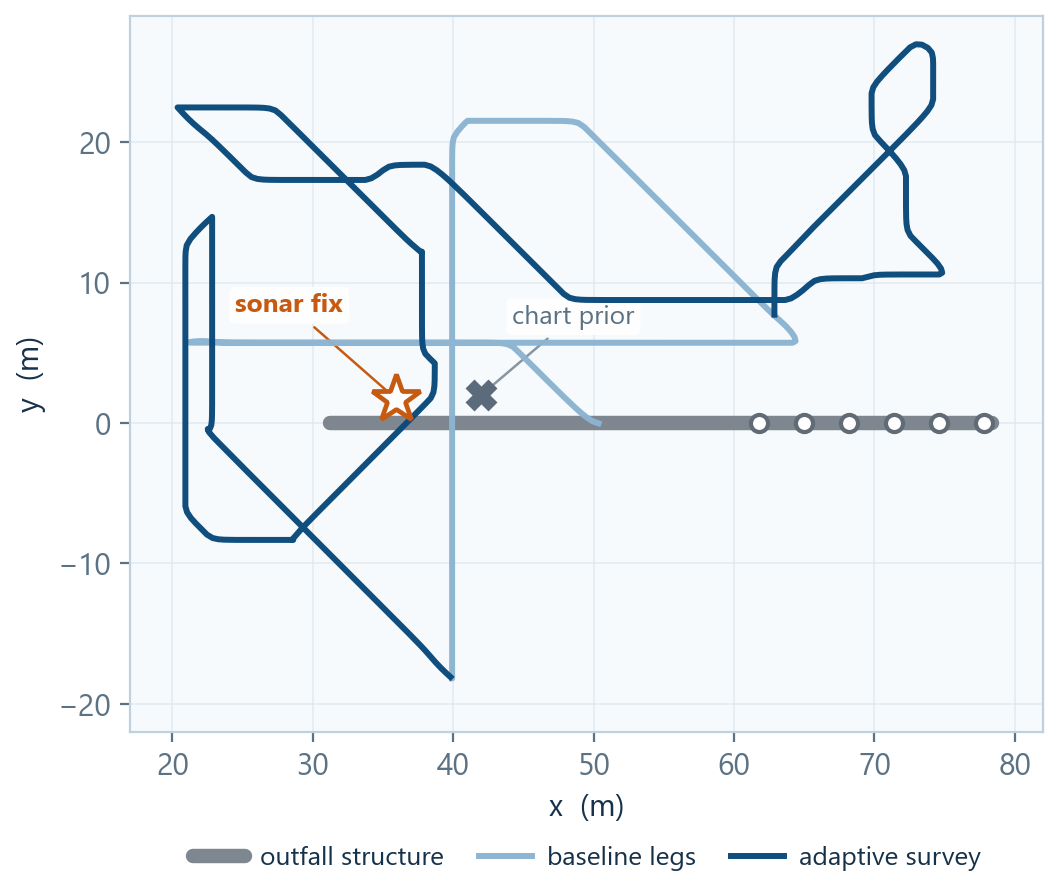
\includegraphics[width=0.84\textwidth]{figures/mission_map.png}
\caption{\textbf{In-engine navigation sequence.} Sonar localisation, baseline legs and adaptive
survey around the outfall.}
\label{fig:mission-map}
\end{figure}

\subsection{A controlled demonstration of the science}

Figure~\ref{fig:reconstruction} compares a known analytic plume on the left with the field
reconstructed by BrineWatch from 591 samples in the same controlled mission on the right. The
white line is the robot trajectory, the orange contour is the boundary estimated by the system and
the dashed dark contour is the known threshold boundary. The reconstruction recovers the plume's
elongated footprint and keeps the less-observed outer areas visibly less regular instead of
presenting them as equally certain. In this scenario the estimated boundary extends beyond the
screening contour, so the system correctly returns \metric{POSSIBLE EXCEEDANCE}. This demonstrates
the complete mapping and screening chain under controlled conditions.

\begin{figure}[t!]
\centering
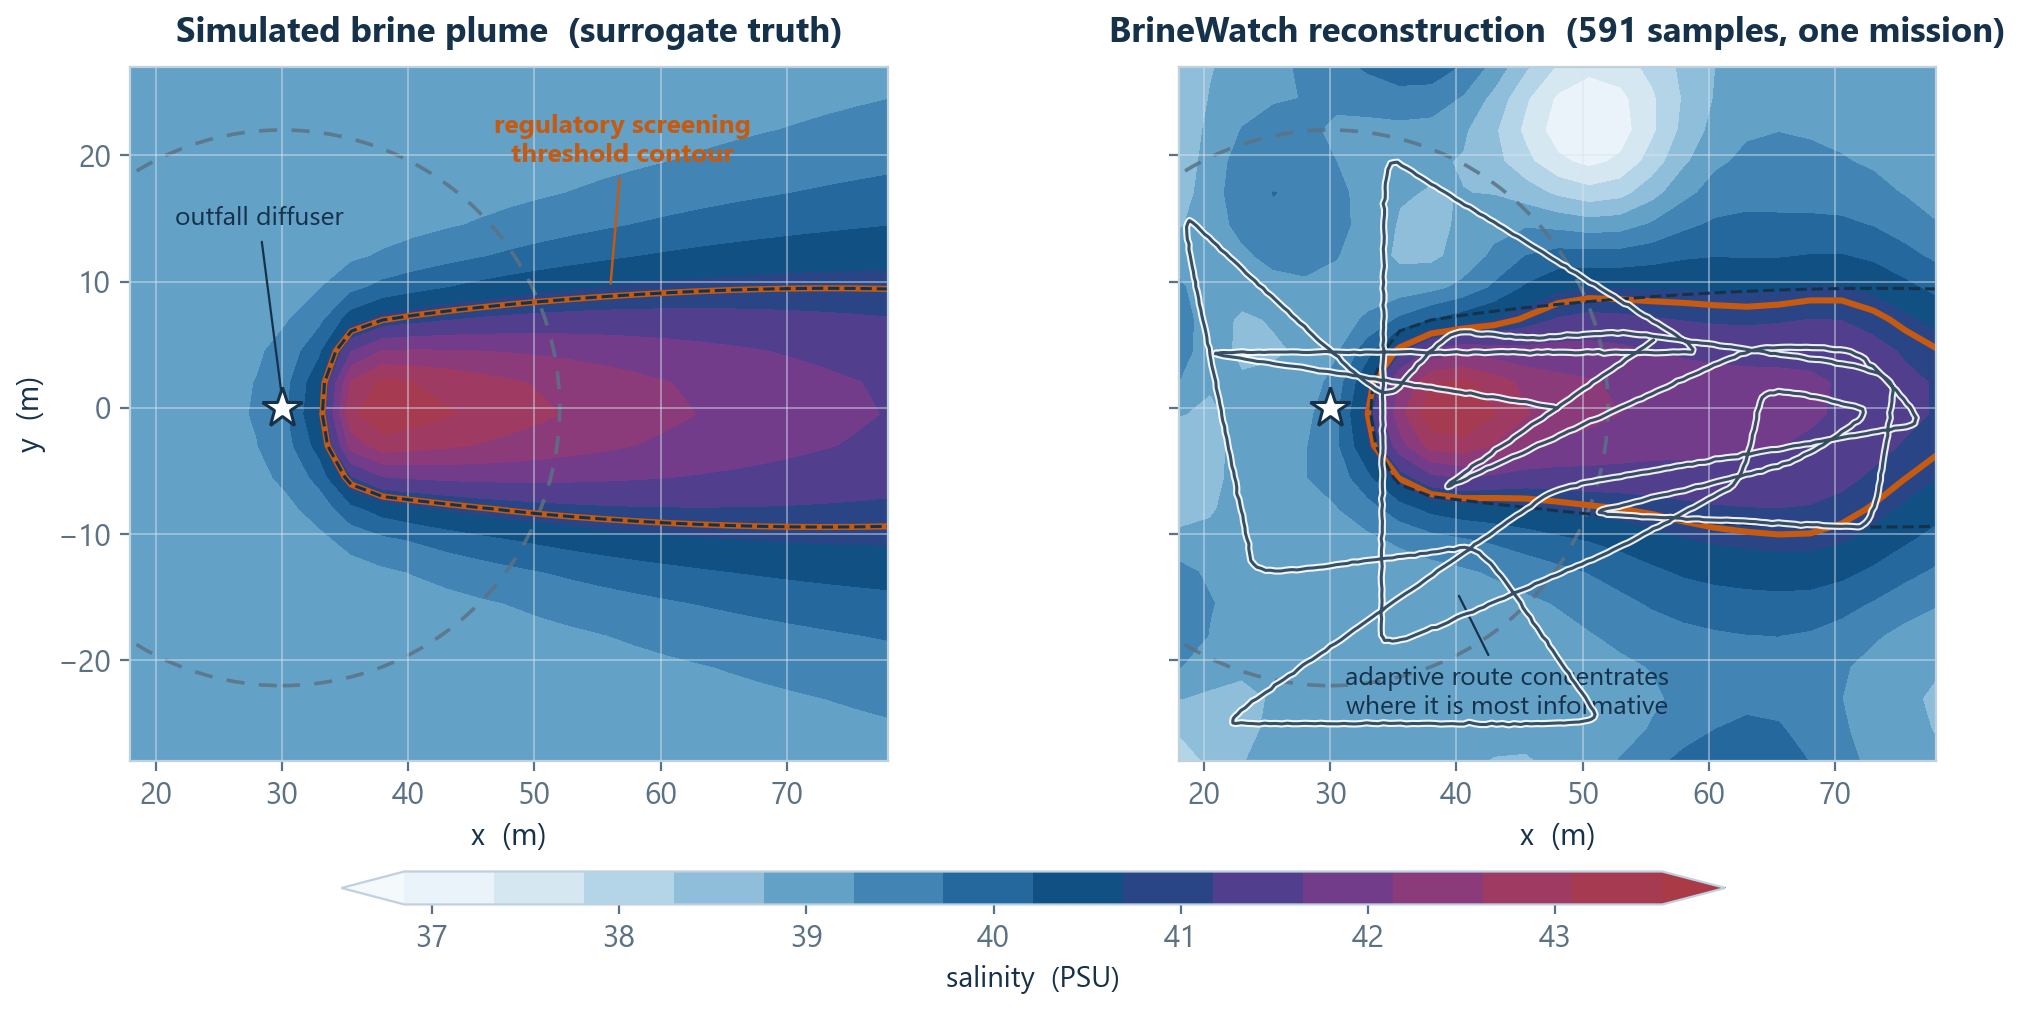
\includegraphics[width=\textwidth]{figures/flagship_2d.png}
\caption{\textbf{Controlled plume reconstruction from 591 samples.}}
\label{fig:reconstruction}
\end{figure}

\subsection{The plume as a volume}

Because brine hugs the seabed, a single-depth map can miss its vertical structure.
Figure~\ref{fig:volume} extends the same controlled scenario into three dimensions using 912
samples collected across four altitude bands from 0.8 to 4.5 m above the bed. The grey bar marks
the diffuser, the thin lines show the four survey paths and the coloured cells are the reconstructed
water volume above the screening threshold. The densest region remains close to the seabed and
narrows with height, while sparse areas away from the sampled bands remain visibly uncertain. The
model reconstructs 2{,}051 m\textsuperscript{3} of above-threshold water against a simulated truth
of 2{,}448 m\textsuperscript{3}, with a volume overlap of 0.81 / 1 and a typical salinity error of
0.48 PSU.

\begin{figure}[h!]
\centering
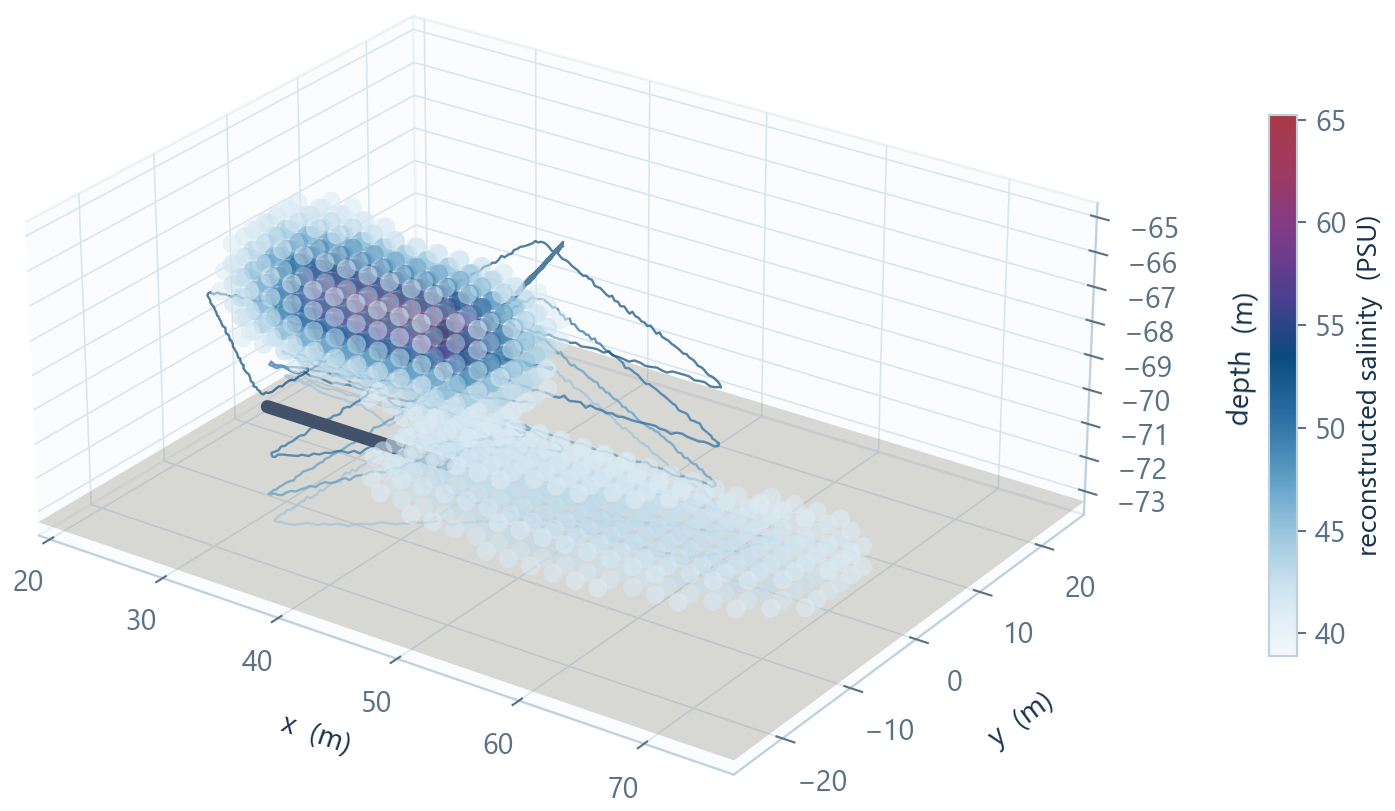
\includegraphics[width=0.72\textwidth]{figures/vol3d.png}
\caption{\textbf{Three-dimensional plume reconstruction from four survey altitudes.}}
\label{fig:volume}
\end{figure}

\clearpage
% ============================================================
% PAGE 9 — ADAPTIVE BENCHMARK + FEASIBILITY (start)
% ============================================================
\section{Why the adaptive route matters}

Is the adaptive planner actually worth it? We tested exactly this with an equal-evidence
benchmark: \keyword{same simulated plume, same 48 readings, same 300 m travel budget and eight
repetitions per method}. Only the sampling strategy differs.

Figure~\ref{fig:benchmark} shows the outcome. Sparse fixed stations produced 17\% useful readings
and no conclusive missions. The regular survey pattern increased this to 23\% useful readings and
four conclusive missions out of eight. The adaptive route concentrated 70\% of its readings in the
informative region, reduced the unresolved plume area to 28\% and produced eight conclusive
missions out of eight. The paths are illustrative, while the percentages and mission counts are
computed benchmark results. No method produced a false \metric{CLEAR}.

\begin{figure}[h!]
\centering
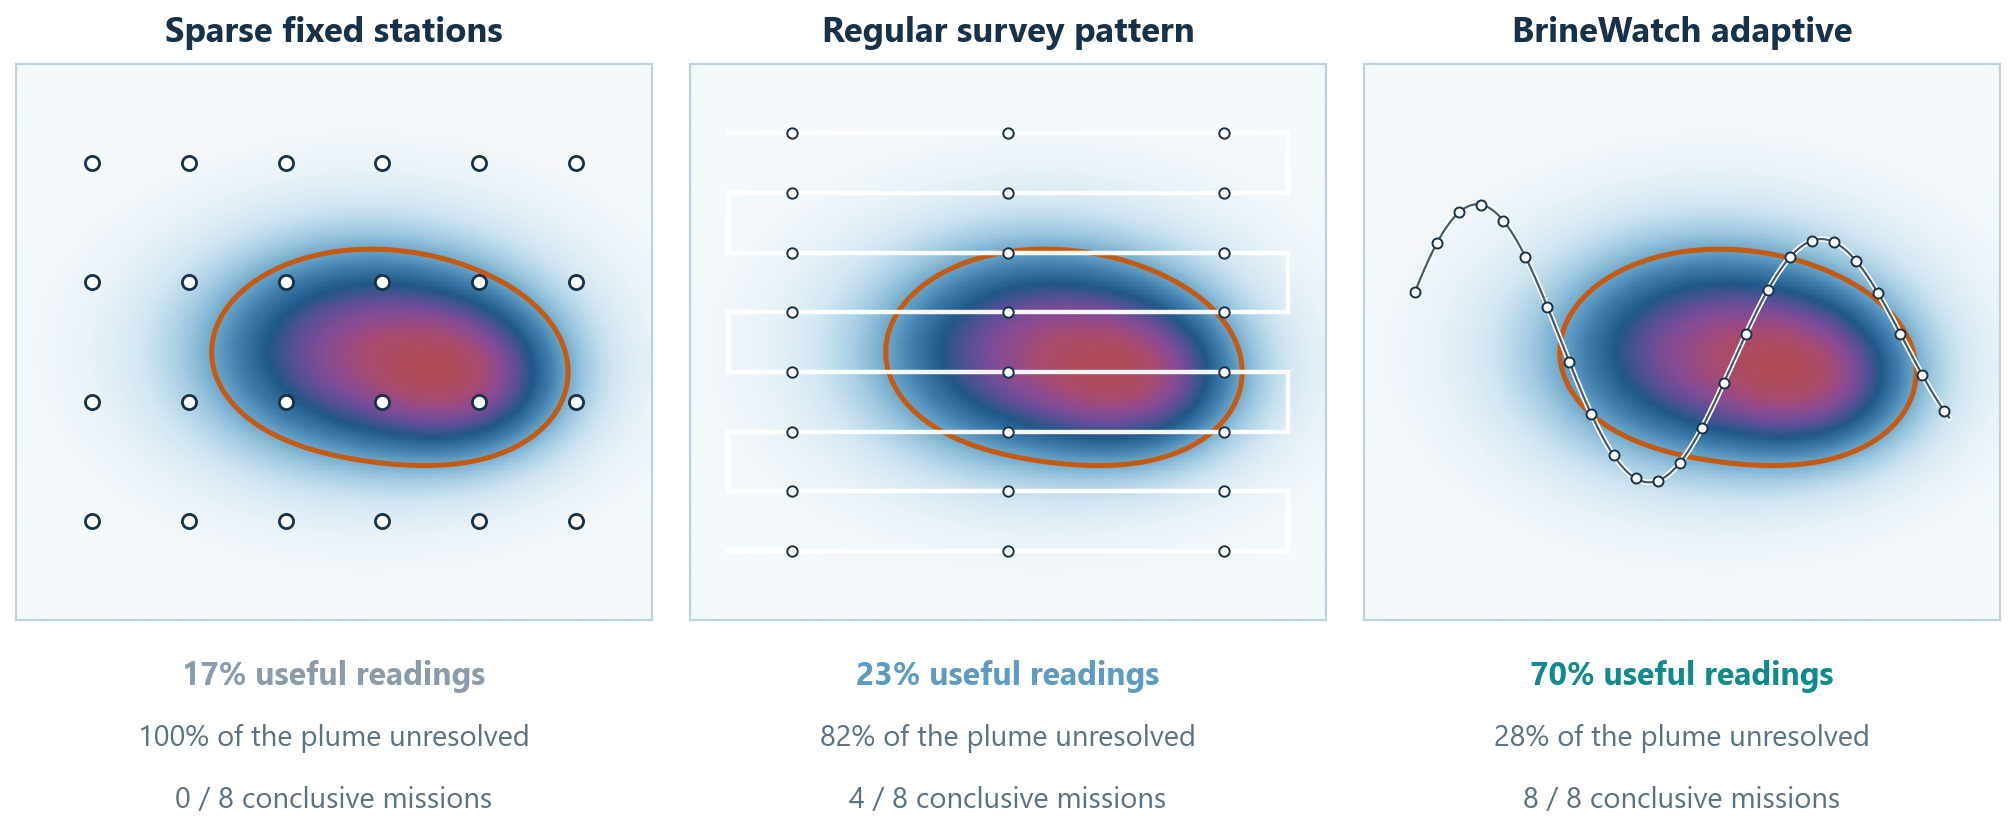
\includegraphics[width=\textwidth]{figures/benchmark.png}
\caption{\textbf{Equal-evidence comparison of three sampling strategies.}}
\label{fig:benchmark}
\end{figure}

% ============================================================
% FEASIBILITY (continues on next page)
% ============================================================
\section{Technical feasibility}

BrineWatch was designed backwards from feasibility: standard vehicle, commercial sonar, one
low-risk scientific sensor and software that is already written and exercised. What separates
today's prototype from a sea-going instrument is integration and validation.

\noindent
\begin{minipage}[t]{0.485\textwidth}
\begin{tealpanel}[height=4.95cm,valign=top]
{\sffamily\bfseries\color{teal}EXISTS AND WORKS TODAY}\\[3pt]
\small
\begin{itemize}
  \item BlueROV2 (owned); Omniscan 450 FS selected, commercially available
  \item custom simulation environment with native imaging sonar
  \item sonar localisation with a 2.35 m error
  \item collision-safe adaptive mission planning
  \item 2-D + 3-D reconstruction with uncertainty
  \item digital twin with three-state screening
  \item mission video and full evaluation package
\end{itemize}
\end{tealpanel}
\end{minipage}\hfill
\begin{minipage}[t]{0.485\textwidth}
\begin{warmpanel}[height=4.95cm,valign=top]
{\sffamily\bfseries\color{accent}NEXT STEPS TOWARDS FIELD DEPLOYMENT}\\[3pt]
\small
\begin{itemize}
  \item calibrated CT sensor integration
  \item time synchronisation and calibration
  \item controlled-water and harbour validation
  \item permits, site access and nearshore pilot partner
\end{itemize}
\end{warmpanel}
\end{minipage}

\subsection*{\sffamily\color{deepblue}Readiness, honestly stated}

The software stack is mission-complete in simulation. The hardware platform is proven
commercial equipment. A calibrated CT sensor is standard oceanographic equipment, but
\emph{integrating and validating} it is exactly
the work the next phase funds. Simulation results use an analytic plume surrogate, not CFD or
field truth: the entire purpose of the roadmap is to replace that surrogate with real water,
step by step.

\subsection*{\sffamily\color{deepblue}Main risks and how we contain them}

\begin{center}
\small\sffamily
\renewcommand{\arraystretch}{1.5}
\begin{tabularx}{\textwidth}{@{}p{3.8cm}cc>{\raggedright\arraybackslash}X@{}}
\toprule
\textbf{\color{deepblue}Risk} & \textbf{\color{deepblue}Likelihood} & \textbf{\color{deepblue}Impact} & \textbf{\color{deepblue}Mitigation}\\
\midrule
CT calibration drift & \chipM & \chipH & Bench and controlled-water calibration; cross-checks with a reference probe during each campaign\\
Sonar localisation in clutter & \chipM & \chipM & Multi-radius consensus already implemented; operator-assisted anchoring available as a fallback\\
Water turbidity & \chipM & \chipL & The mission relies primarily on sonar; the camera is secondary\\
Currents and station keeping & \chipM & \chipM & Heavier vehicle configuration, conservative survey speeds and predefined abort thresholds\\
Navigation near the structure & \chipL & \chipH & Collision-safe planner validated in simulation, with zero collisions and four safe detours; conservative standoff distance\\
Regulatory approval and site access & \chipM & \chipH & Early engagement with utilities and regulators; harbour trials can proceed without access to an operating outfall\\
Field reference sampling & \chipL & \chipM & The pilot budget includes independent certified reference measurements\\
\bottomrule
\end{tabularx}
\end{center}

\begin{panel}
\small\sffamily \textbf{\color{deepblue}Scope statement.}\ BrineWatch is a screening and targeting
instrument on a path to controlled-water and nearshore validation. It is not a certified
compliance system. Simulation results are not field measurements; they demonstrate the
instrument, not the ocean.
\end{panel}

% ============================================================
% PAGE 10 — COST, MANAGEMENT, ROADMAP
% ============================================================
\section{Cost, management and roadmap}

\subsection*{\sffamily\color{deepblue}Reusable system, low-cost repeat missions}

BrineWatch separates the one-time cost of completing the robotic system from the much lower cost
of repeating a mission. It is completed once and reused: subsequent missions require no dedicated
survey vessel and produce a precise spatial map rather than a limited set of isolated measurements.

After the initial investment, recurring costs are limited to local transport, consumables,
equipment wear and the internal operational team. When needed, a small local boat can be rented
for a short deployment. BrineWatch does not require the purchase or permanent operation of a fully
equipped survey vessel.

\begin{center}
\small\sffamily
\renewcommand{\arraystretch}{1.34}
\begin{tabularx}{\textwidth}{@{}>{\raggedright\arraybackslash}p{4.0cm}>{\raggedright\arraybackslash}p{4.0cm}>{\raggedright\arraybackslash}X@{}}
\toprule
\textbf{\color{deepblue}Cost model} & \textbf{\color{deepblue}Indicative cost} & \textbf{\color{deepblue}Main result}\\
\midrule
\rowcolor{panelblue}
\textbf{One-time system completion} & \textbf{USD 5k--9k once} & Reusable ROV, sonar, CT payload and digital-twin system\\
\rowcolor{panelteal}
\textbf{Repeated BrineWatch mission} & \textbf{USD 150--500 from shore; USD 1k--2.5k with a small chartered boat} & Inspection, adaptive measurements, plume map, uncertainty and site-history update\\
\rowcolor{panelwarm}
\textbf{Fully equipped research vessel} & \textbf{USD 20.5k--24.5k per day, vessel only} & Conventional ship-based survey\\
\bottomrule
\end{tabularx}
\end{center}

\noindent
\begin{minipage}[t]{0.485\textwidth}
\begin{panel}[height=5.35cm,valign=top]
{\sffamily\bfseries\color{deepblue}ONE-TIME SYSTEM COMPLETION}\\[2pt]
{\sffamily\bfseries\color{deepblue}USD 5k--9k}\\[4pt]
\small Omniscan 450 FS, calibrated CT payload, mounting and interfaces, integration, calibration
and essential spares. Once completed, the same system can be reused across repeated missions.

\vspace{5pt}
{\sffamily\bfseries\color{teal}REPEATED BRINEWATCH MISSION}\\[2pt]
{\small\sffamily\bfseries\color{teal}USD 150--500 from shore\\USD 1k--2.5k with a small chartered boat}
\end{panel}
\end{minipage}\hfill
\begin{minipage}[t]{0.485\textwidth}
\begin{warmpanel}[height=5.35cm,valign=top]
{\sffamily\bfseries\color{accent}CONVENTIONAL VESSEL CAMPAIGN}\\[2pt]
{\sffamily\bfseries\color{accent}USD 20.5k--24.5k per day}\\
{\footnotesize\sffamily\color{muted}for the research vessel alone}\\[4pt]
\small Published 2026 rates for fully equipped research vessels are approximately USD
20.5k--24.5k per day, before additional scientific personnel, laboratory analysis, permits and
reporting~[7].
\end{warmpanel}
\end{minipage}

\newpage
\subsection*{\sffamily\color{deepblue}Lower cost without sacrificing spatial evidence}

BrineWatch's advantage is not only economic. One mission combines outfall localisation,
infrastructure inspection, adaptive environmental measurements, 2-D and 3-D plume reconstruction,
uncertainty estimation and a digital-twin update.

In the controlled simulation benchmark, BrineWatch achieved a plume-boundary score of
\metric{0.95/1}, a 2-D overlap of \metric{0.90/1} and a salinity reconstruction error of
\metric{0.34 PSU}. The 3-D reconstruction achieved an overlap of \metric{0.81/1} with an error of
\metric{0.48 PSU}.

These results demonstrate high reconstruction accuracy in controlled simulation. Field accuracy
will be independently validated during controlled-water and nearshore trials.

\subsection*{\sffamily\color{deepblue}Development roadmap with decision gates}

\begin{center}
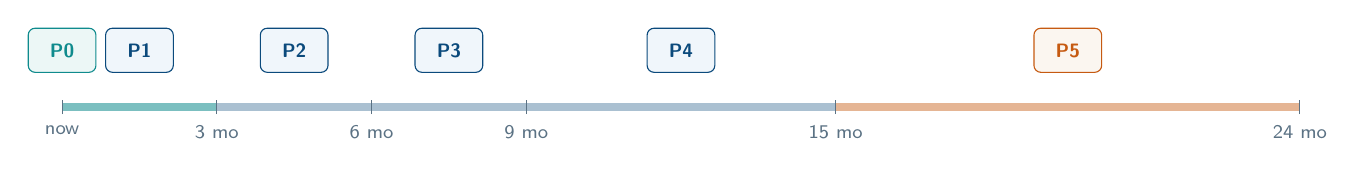
\begin{tikzpicture}[font=\scriptsize\sffamily,x=0.655cm]
  \draw[hairline,line width=1.5pt] (0,0) -- (24,0);
  \draw[teal!55,line width=2.6pt] (0,0) -- (3,0);
  \draw[deepblue!35,line width=2.6pt] (3,0) -- (15,0);
  \draw[accent!45,line width=2.6pt] (15,0) -- (24,0);
  \foreach \x/\lab in {0/now,3/3 mo,6/6 mo,9/9 mo,15/15 mo,24/24 mo}{
    \draw[muted] (\x,-0.09) -- (\x,0.09);
    \node[below,color=muted] at (\x,-0.12) {\lab};}
  \newcommand{\phasebox}[4]{
    \node[draw=#3,fill=#4,rounded corners=2.5pt,align=center,
          minimum width=0.86cm,minimum height=0.56cm,inner sep=2pt]
          at (#1,0.72) {\textbf{\color{#3}#2}};}
  \phasebox{0}{P0}{teal}{panelteal}
  \phasebox{1.5}{P1}{deepblue}{panelblue}
  \phasebox{4.5}{P2}{deepblue}{panelblue}
  \phasebox{7.5}{P3}{deepblue}{panelblue}
  \phasebox{12}{P4}{deepblue}{panelblue}
  \phasebox{19.5}{P5}{accent}{panelwarm}
\end{tikzpicture}
\end{center}

\vspace{-2pt}
\begin{itemize}\small
  \item \keyword{P1: CT payload integration} (0--3 mo): sensor, mounting, power, time sync and bench calibration. \emph{Main cost: sensor + integration.}
  \item \keyword{P2: Controlled water} (3--6 mo): known salinity gradients, independent truth samples, reconstruction-error validation and repeatability. \emph{Main cost: facility time.}
  \item \keyword{P3: Harbour / sheltered water} (6--9 mo): navigation robustness, sonar localisation on real structures and surrogate plume-release experiments. \emph{Main cost: operations.}
  \item \keyword{P4: Supervised nearshore pilot} (9--15 mo): a real outfall inspection with certified reference samples and operator feedback. \emph{Main cost: vessel, permits and reference lab.}
  \item \keyword{P5: Repeat monitoring} (15--24 mo): scheduled campaigns, trends in the twin and service definition. \emph{Main cost: campaign operations.}
\end{itemize}

% ============================================================
% PAGES 11--12 — APPLICATIONS, IMPACT, REQUEST
% ============================================================
\section{Applications, impact and what support unlocks}

\noindent
\begin{minipage}[t]{0.485\textwidth}
\begin{tealpanel}
{\sffamily\bfseries\color{teal}PRIMARY APPLICATIONS}\\[3pt]
\small
\begin{itemize}
  \item desalination outfall inspection
  \item brine-plume screening around diffusers
  \item targeting of certified environmental sampling
  \item repeated digital site history per outfall
\end{itemize}
\end{tealpanel}
\end{minipage}\hfill
\begin{minipage}[t]{0.485\textwidth}
\begin{panel}
{\sffamily\bfseries\color{deepblue}THE SAME INSTRUMENT ALSO SERVES}\\[3pt]
\small
\begin{itemize}
  \item wastewater outfalls and industrial discharge points
  \item desalination intakes and their protection zones
  \item harbour and coastal infrastructure inspection
  \item research monitoring of benthic habitats
\end{itemize}
\end{panel}
\end{minipage}

\subsection*{\sffamily\color{deepblue}Impact, in four dimensions}

\small
\begin{tabularx}{\textwidth}{@{}p{2.6cm}>{\raggedright\arraybackslash}X@{}}
\textbf{\color{teal}Environmental} & seabed conditions become visible; certified sampling lands where it matters; anomalies surface earlier, between formal campaigns.\\[4pt]
\textbf{\color{teal}Operational} & inspection and environmental screening merge into one mission; site understanding same-day instead of next-quarter; a procedure any trained ROV crew can repeat.\\[4pt]
\textbf{\color{teal}Economic} & reuses robotic hardware many operators already own; fewer blind sampling stations; growing value of an accumulated site history.\\[4pt]
\textbf{\color{teal}Scientific} & a working bridge between CFD predictions, robotic measurement and field validation, with a reusable architecture for underwater environmental monitoring.\\
\end{tabularx}
\normalsize

\subsection*{\sffamily\color{deepblue}What support would enable}

\begin{panel}
\small With the resources of the next validation gate (Section 8), the team will: integrate and
calibrate the \keyword{CT payload}; validate reconstruction accuracy in \keyword{controlled
water} against independent truth; run \keyword{harbour trials}; and prepare a
\keyword{supervised nearshore pilot} at an outfall with certified reference sampling.
\end{panel}

\vspace{6pt}
\begin{center}
{\fontsize{13}{17}\selectfont\itshape\color{deepblue}%
BrineWatch is ready to move from simulation-led evidence\\to controlled-water and nearshore validation.}
\end{center}

\noindent
\begin{minipage}{\textwidth}
\centering
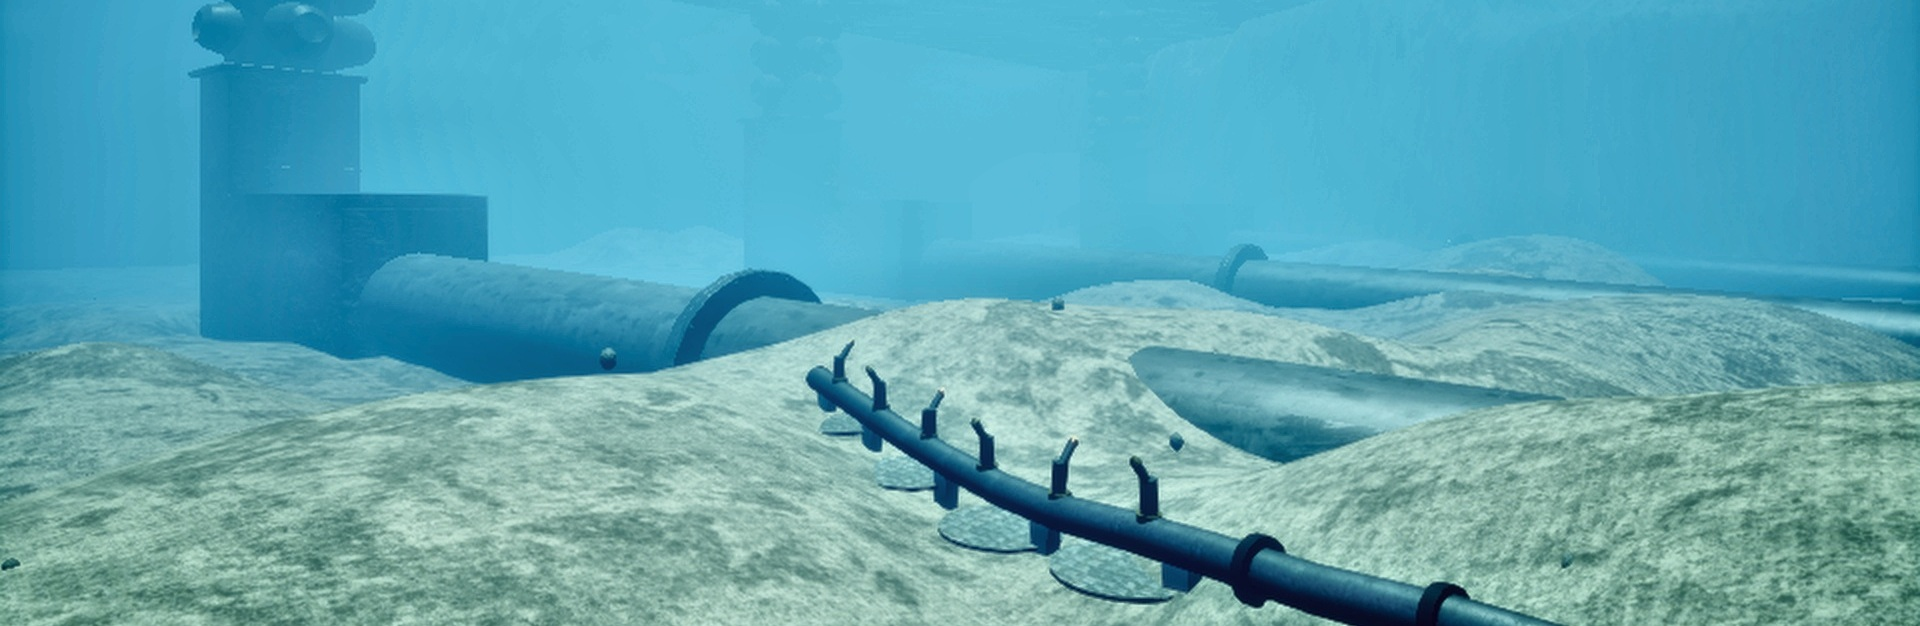
\includegraphics[width=\textwidth]{figures/closing_banner.jpg}\par
\vspace{5pt}
{\small\color{muted}Our outfall site in the simulation.}
\end{minipage}

\vspace{7pt}
{\sffamily\small\color{navy}\textbf{Andrea Bedei} \textperiodcentered\ University of Bologna \textperiodcentered\
supervisors Roberto Girau \& Giovanni Pau \textperiodcentered\
Prototypes for Humanity 2026}

\vspace{4pt}
{\color{hairline}\hrule height 0.8pt}
\vspace{4pt}
{\footnotesize\color{muted}
[1] E.~Jones \emph{et al.}, ``The state of desalination and brine production: a global outlook,'' \emph{Sci.\ Total Environ.}~657, 2019.\par
[2] P.\,J.\,W.~Roberts, ``Near-field flow dynamics of concentrate discharges and diffuser design,'' in \emph{Intakes and Outfalls for Seawater RO Desalination}, Springer, 2015.\par
[3] G.~Hitz \emph{et al.}, ``Adaptive continuous-space informative path planning for online environmental monitoring,'' \emph{J.~Field Robotics} 34(8), 2017.\par
[4] E.~Potokar \emph{et al.}, ``HoloOcean: an underwater robotics simulator,'' \emph{IEEE ICRA}, 2022; ``A preview of HoloOcean 2.0,'' arXiv:2510.06160, 2025.\par
[5] Blue Robotics: BlueROV2 product page, price checked 22 July 2026.\par
[6] Cerulean Sonar: Omniscan 450 FS product page, price checked 22 July 2026.\par
[7] Marine Institute: 2026 vessel rates of EUR 18{,}000--21{,}500 per day; converted at the ECB
reference rate of USD 1.1426 per EUR, 20 July 2026.\par
[8] BrineWatch project video: \url{https://youtu.be/bsZbojE48Yk}.\par
All performance figures in this document are simulation results, reproduced deterministically from
the project repository; the technical evidence ledger with full metrics and limitations accompanies
this proposal.}

\end{document}
